% 11/23/2015
%%%%%%%%%%%%%%%%%%%%%%%%%%%%%%%%%%%%%%%%%%%%%%%%%%%%%%%%%%%%%%%%%%%%%%%%%%%%
% AGUJournalTemplate.tex: this template file is for articles formatted with LaTeX
%
% This file includes commands and instructions
% given in the order necessary to produce a final output that will
% satisfy AGU requirements. 
%
% You may copy this file and give it your
% article name, and enter your text.
%
%%%%%%%%%%%%%%%%%%%%%%%%%%%%%%%%%%%%%%%%%%%%%%%%%%%%%%%%%%%%%%%%%%%%%%%%%%%%
% PLEASE DO NOT USE YOUR OWN MACROS
% DO NOT USE \newcommand, \renewcommand, or \def, etc.
%
% FOR FIGURES, DO NOT USE \psfrag or \subfigure.
% DO NOT USE \psfrag or \subfigure commands.
%%%%%%%%%%%%%%%%%%%%%%%%%%%%%%%%%%%%%%%%%%%%%%%%%%%%%%%%%%%%%%%%%%%%%%%%%%%%
%
% All questions should be e-mailed to latex@agu.org.
%
%%%%%%%%%%%%%%%%%%%%%%%%%%%%%%%%%%%%%%%%%%%%%%%%%%%%%%%%%%%%%%%%%%%%%%%%%%%%
%
% Step 1: Set the \documentclass
%
% There are two options for article format:
%
% 1) PLEASE USE THE DRAFT OPTION TO SUBMIT YOUR PAPERS.
% The draft option produces double spaced output.
% 
% 2) numberline will give you line numbers.

%% To submit your paper:
\documentclass[draft,linenumbers]{agujournal}
\draftfalse

%% For final version.
%\documentclass{agujournal}
\usepackage{url}
%\newcommand*{\gi}[1]{\overline{\overline{#1}}}
\newcommand*{\gi}[1]{\widehat{#1}}
\usepackage{graphicx}%for gnuplot epslatex
% Now, type in the journal name: \journalname{<Journal Name>}

% ie, \journalname{Journal of Geophysical Research}
%% Choose from this list of Journals:
%
% JGR-Atmospheres
% JGR-Biogeosciences
% JGR-Earth Surface
% JGR-Oceans
% JGR-Planets
% JGR-Solid Earth
% JGR-Space Physics
% Global Biochemical Cycles
% Geophysical Research Letters
% Paleoceanography
% Radio Science
% Reviews of Geophysics
% Tectonics
% Space Weather
% Water Resource Research
% Geochemistry, Geophysics, Geosystems
% Journal of Advances in Modeling Earth Systems (JAMES)
% Earth's Future
% Earth and Space Science
%
%

\journalname{Journal of Advances in Modeling Earth Systems (JAMES)}


\begin{document}

%% ------------------------------------------------------------------------ %%
%  Title
% 
% (A title should be specific, informative, and brief. Use
% abbreviations only if they are defined in the abstract. Titles that
% start with general keywords then specific terms are optimized in
% searches)
%
%% ------------------------------------------------------------------------ %%

% Example: \title{This is a test title}

\title{A total energy error analysis of dynamical cores and physics-dynamics coupling in the Community Atmosphere Model (CAM)}

%% ------------------------------------------------------------------------ %%
%
%  AUTHORS AND AFFILIATIONS
%
%% ------------------------------------------------------------------------ %%

% Authors are individuals who have significantly contributed to the
% research and preparation of the article. Group authors are allowed, if
% each author in the group is separately identified in an appendix.)

% List authors by first name or initial followed by last name and
% separated by commas. Use \affil{} to number affiliations, and
% \thanks{} for author notes.  
% Additional author notes should be indicated with \thanks{} (for
% example, for current addresses). 

% Example: \authors{A. B. Author\affil{1}\thanks{Current address, Antartica}, B. C. Author\affil{2,3}, and D. E.
% Author\affil{3,4}\thanks{Also funded by Monsanto.}}

\authors{Peter H. Lauritzen\affil{1}\thanks{1850 Table Mesa Drive, Boulder, Colorado, USA}, and David .L. Williamson \affil{1}}

 \affiliation{1}{National Center for Atmospheric Research, Boulder, Colorado, USA}
% \affiliation{2}{School of Marine and Atmospheric Sciences, Stony Brook University, State University of New York, Stony Brook, New York}
% \affiliation{3}{Sandia National Laboratories, Albuquerque, New Mexico, USA}
% \affiliation{4}{Department of Land, Air and Water Resources, University of California, Davis, California, USA}
% \affiliation{5}{Ecole Polytechnique, UMR 8539, Laboratoire de M\'et\'eorologie Dynamique/IPSL, Palaiseau, France}
% \affiliation{6}{Rosenstiel School of Marine and Atmospheric Science, University of Miami, Miami, Florida, USA}

% \affiliation{3}{Third Affiliation}
% \affiliation{4}{Fourth Affiliation}

%(repeat as many times as is necessary)

%% Corresponding Author:
% Corresponding author mailing address and e-mail address:

% (include name and email addresses of the corresponding author.  More
% than one corresponding author is allowed in this LaTeX file and for
% publication; but only one corresponding author is allowed in our
% editorial system.)  

% Example: \correspondingauthor{First and Last Name}{email@address.edu}

\correspondingauthor{Peter Hjort Lauritzen}{pel@ucar.edu}

%% Keypoints, final entry on title page.

% Example: 
 \begin{keypoints}
 \item Spurious total energy dissipation in dynamical core is $-0.3W/m^2$ to $-1W/m^2$ at 1 degree
 \item Constant-pressure assumption in physics leads to $0.3W/m^2$ spurious total energy source
 \item There can easily be compensating errors in total energy budget
%               x         x         x         x         x         x         x         x         x         x100
% \item Limiters on vertical remapping increase TE dissipation to $-0.2W/m^2$
% \item Moist physics forcing increases spurious TE  dissipation in dynamical core

% \item Physics-dynamics coupling can lead to $0.5W/m^2$ spurious TE source
% \item Physics-dynamics coupling can lead to noisy solutions for large physics time-steps
% \item Vertical remapping TE dissipation is $-0.01W/m^2$
%

% \item Total energy analysis in simplified setups (such as aqua-planet or Held-Suarez) does not give an accurate picture of TE dissipation in AMIP-type simulations

% \item	List up to three key points (at least one is required)
% \item	Key Points summarize the main points and conclusions of the article
% \item	Each must be 100 characters or less with no special characters or punctuation 
 \end{keypoints}

%  List up to three key points (at least one is required)
%  Key Points summarize the main points and conclusions of the article
%  Each must be 100 characters or less with no special characters or punctuation 

%% ------------------------------------------------------------------------ %%
%
%  ABSTRACT
%
% A good abstract will begin with a short description of the problem
% being addressed, briefly describe the new data or analyses, then
% briefly states the main conclusion(s) and how they are supported and
% uncertainties. 
%% ------------------------------------------------------------------------ %%

%% \begin{abstract} starts the second page 

\begin{abstract}
A closed total energy (TE) budget is of utmost importance in coupled climate system modeling; in particular, the dynamical core or physics-dynamics coupling should ideally not lead to spurious TE sources/sinks. To assess this in a global climate model, a detailed analysis of the spurious sources/sinks of TE in NCAR's Community Atmosphere Model (CAM) is given. This includes spurious sources/sinks associated with the parameterization suite, the dynamical core, TE definition discrepancies and physics-dynamics coupling.  The latter leads to a  detailed discussion of the pros and cons of various physics-dynamics coupling methods commonly used in climate/weather modeling.  

%It is shown that the dynamical core dissipates energy at $-0.3W/m^2$ to $1W/m^2$ depending on configuration and numerical methods at $1^\circ$ resolution. Most TE dissipation comes viscosity. Shape-preserving limiters on the vertical remapping used in quasi-Lagrangian vertical coordinate models increase TE dissipation of the mapping from $-0.01W/m^2$ $-0.2W/m^2$. TE dissipation in dynamical core increases drastically with rougher topography and the inclusion of moist physics. Hence TE analysis of simplified (in particular dry) setups does not necessarily provide a good estimate of the TE budget under `real-world' conditions. Physics-dynamics coupling can be a $0.5W/m^2$ TE source and the constant-pressure assumption along with the requirement for a closed mass budget leads to a $0.3W/m^2$ TE source.
\end{abstract}


%% ------------------------------------------------------------------------ %%
%
%  TEXT
%
%% ------------------------------------------------------------------------ %%

%%% Suggested section heads:
%\section{Introduction}
% 
% The main text should start with an introduction. Except for short
% manuscripts (such as comments and replies), the text should be divided
% into sections, each with its own heading. 

% Headings should be sentence fragments and do not begin with a
% lowercase letter or number. Examples of good headings are:

% \section{Materials and Methods}
% Here is text on Materials and Methods.
%
% \subsection{A descriptive heading about methods}
% More about Methods.
% 
% \section{Data} (Or section title might be a descriptive heading about data)
% 
% \section{Results} (Or section title might be a descriptive heading about the
% results)
% 
% \section{Conclusions}


\section{Introduction}
In coupled climate modeling with prognostic atmosphere, ocean, land, land-ice, and sea-ice components, it is important to conserve total energy (TE) to a high degree in each component individually and in the complete model to avoid spurious long term trends in the simulated Earth system. Conservation of TE in this context refers to having a closed TE budget. For example, the TE change in a column in the atmosphere is exactly balanced by the net sources/sinks given by the fluxes through the column. The fluxes into the atmospheric component from the surface models must be balanced by the fluxes in the respective surface components and so on. Henceforth we will focus only on the atmospheric component which, in a numerical model, is split into a resolved-scale component (the dynamical core) and a sub-grid-scale component (parameterizations or, in modeling jargon, physics). While there have been many studies on energy flow in the Earth system through analysis of re-analysis data and observations \citep[][and references herein]{TF2018JC}, there has been less focus on spurious TE sources/sinks in numerical models.

The atmospheric equations of motion conserve TE but the discretizations used in climate and weather models are usually not inherently TE conservative. Exact conservation is probably not necessary but conservation to within $\sim $0.01  $W/m^2$ has been considered sufficient to avoid spurious trends in century long simulations \citep{B2000S,WOHTTV2015JAMES}. Spurious sources and sinks of TE can be introduced by the dynamical core, physics, physics-dynamics coupling as well as discrepancies between the TE of the continuous and discrete equations of motion and for the physics. Hence the study of TE conservation in comprehensive models of the atmosphere quickly becomes a quite complex and detailed matter. In addition there can easily be compensating errors in the system as a whole.

Here we focus on versions of the Community Atmosphere Model (CAM) that use the spectral-element \citep[SE, ][]{LetAl2018JAMES} and finite-volume \citep[FV, ][]{L2004MWR} dynamical cores. These dynamical cores couple with physics in a time-split manner, i.e. physics receives a state updated by dynamics \citep[see ][ for a discussion of time-split versus process split physics-dynamics coupling in the context of CAM]{W2002MWR}. In its pure time-split form the physics tendencies are added to the state previously produced by the dynamical core and the resulting state provides the initial state for the subsequent dynamical core calculation. We refer to this as {\em{state-updating}} ({\tt{ftype=1}} in CAM code). Alternatively, when the dynamical core adopts a shorter time step than the physics, say {\tt{nsplit}} sub-steps, then (1/{\tt{nsplit}})th of the physics-calculated tendency is added to the state before each dynamics sub-step. We refer to this modification of time-splitting as {\em{dribbling}} ({\tt{ftype=0}}). CAM-FV uses the {\em{state-update}} ({\tt{ftype=1}}) approach while CAM-SE has options to use {\em{state-update}} ({\tt{ftype=1}}), {\em{dribbling}} ({\tt{ftype=0}}) or a combination of the two i.e. mass-variables use {\em{state-updating}} and remaining variables use {\em{dribbling}}. We refer to this as {\em{combination}} ({\tt{ftype=2}}). The {\em{dribbling}} variants can lead to spurious sources or sinks of TE (and mass) referred to here as physics-dynamics coupling errors.

The dynamical core usually has inherent or specified filters to control spurious noise near the grid scale which will lead to energy dissipation \citep{T2008JCP,JW2010LNCSE}. Similarly models often have sponge layers to control the solution near the top of the model that may be a sink of TE. There are examples of numerical discretizations of the adiabatic frictionless equations motion that are designed so that TE is conserved in the absence of time-truncation and filtering errors \citep[e.g., ][]{ER2017GMD,MC2013QJRMS}, e.g., mimetic spectral-element discretizations such as the one used in the horizontal in CAM-SE \citep{T2011LNCSEb}. These provide consistency between the discrete momentum and thermodynamic equations leading to global conservation associated with the conversion of potential to kinetic energy. In spectral transform models it is customary to add the energy change due to explicit diffusion on momentum back as heating (referred to as frictional heating), so that the diffusion of momentum does not affect the TE budget \citep[see, e.g., p.71 in ][]{CAM5}. This is also done in CAM-SE \citep{LetAl2018JAMES}. 

The purpose of this paper is to provide a detailed global TE analysis of CAM. We assess TE errors due to various steps in the model algorithms. The paper is outlined as follows. In section \ref{sec:methods} the continuous TE formulas are given and a detailed description of spurious TE sources/sinks that can occur in a model as a whole, and the associated diagnostics used to perform the TE analysis, are defined. In section \ref{sec:results} the model is run in various configurations to assess their effects on TE conservation. This includes various physics-dynamics coupling experiments leading to a rather detailed discussion of mass budget closure. We also investigate the effect of using a limiter in the vertical remapping of momentum, assess energy discrepancy errors and impacts on TE of simplifying surface conditions and dry atmosphere experiments. The paper ends with conclusions.


%For example, the discrete TE consistent with the dynamical core may differ from the one used in physics or,  even worse, the TE that the continuous equations of motion conserve is different between the dynamical core and physics.\\

\section{Method}
\label{sec:methods}
\subsection{Defining total energy (TE)}\label{sec:defE}
In the following it is assumed that the model top and bottom are coordinate surfaces and that there is no flux of mass through the model top and bottom. In a dry {\color{red}{hydrostatic}} atmosphere the TE equation integrated over the entire sphere is given by
\begin{equation}
\frac{d}{dt}\int_{z=z_s}^{z=z_{top}}\iint_{\mathcal{S}} E_v \rho^{(d)}\, dA\, dz=\int_{z=z_s}^{z=z_{top}}\iint_{\mathcal{S}} F_{net}\, \rho^{(d)} dA\, dz,
\end{equation}
\citep[e.g., ][]{K1974MWR} where $F_{net}$ is net flux calculated by the parameterizations (e.g., heating and momentum forcing), $d/dt$ the total/material derivative, $z_s$ is the height of the surface, $\mathcal{S}$ the sphere, $\rho^{(d)}$ the density of dry air, $E_v$ is the TE and $dA$ is an infinitesimal area on the sphere. $E_v$ can be split into kinetic energy $K=\frac{1}{2}\mathbf{v}^2$ ($\mathbf{v}$ is the wind vector), internal energy $c_v^{(d)}T$, where $c_v^{(d)}$ is the heat capacity of dry air at constant volume, and potential energy $\Phi=gz$
\begin{equation}
E_v=K+c_v^{(d)}T+\Phi.
\end{equation}
If the vertical integral is performed in a mass-based vertical coordinate, e.g., pressure, then the integrated TE equation for a dry atmosphere can be written as
\begin{equation}
\frac{d}{dt}\int_{p=p_s}^{p=p_{top}}\iint_{\mathcal{S}} E_p \, dA\, dp + \frac{d}{dt}\iint_{\mathcal{S}}\Phi_sp_s dA =\int_{p=p_s}^{p=p_{top}}\iint_{\mathcal{S}} F_{net}\, dA\, dp,
\end{equation}
\citep[e.g., ][]{K1974MWR} where
\begin{equation}
E_p=K+c_p^{(d)}T.
\end{equation}
In a moist atmosphere, however, there are several definitions of TE used in the literature related to what heat capacity is used for water vapor and whether or not condensates are accounted for in the energy equation. To explain the details of that we focus on the energy equation for CAM-SE.

CAM-SE is formulated using a terrain-following hybrid-sigma vertical coordinate $\eta$ but the coordinate levels are defined in terms of dry air mass per unit area ($M^{(d)}$) instead of total air mass; $\eta^{(d)}$ \citep[see ][ for details]{LetAl2018JAMES}. In such a coordinate system it is convenient to define the tracer state in terms of a dry mixing ratio instead of moist mixing ratio
\begin{equation}
m^{(\ell)}\equiv \frac{\rho^{(\ell)}}{\rho^{(d)}}, \text{ where }\ell=`wv`,`cl`,`ci`,`rn`,`sw`,\label{eq:mx}
\end{equation}
where $\rho^{(d)}$ is the mass of dry air per unit volume of moist air and $\rho^{(\ell)}$ is the mass of the water substance of type $\ell$ per unit volume of moist air. Moist air refers to air containing dry air (`$d$`), water vapor (`$wv$`), cloud liquid (`$cl$`), cloud ice (`$ci$`), rain amount (`$rn$`) and snow amount (`$sw$`). For notational purposes define the set of all components of air
\begin{equation}
\mathcal{L}_{all}=\left\{ `d`,`wv`,`cl`,`ci`,`rn`,`sw`\right\},
\end{equation}
Define associated heat capacities at constant pressure $c_p^{(\ell)}$. {\color{red}{We refer to condensates as being {\em{thermodynamically and inertially active}} if they are included in the thermodynamic equation and momentum equations. E.g. if the thermodynamic equation is formulated in terms of temperature the energy conversion term includes a generalized heat capacity which is a function of the condensates and their associated heat capacities \citep[see, e.g., section 2.3 in ][]{LetAl2018JAMES}. Similarly the weight of the condensates is included in the pressure field and pressure gradient force.}}  How many and which condensates are thermodynamically{\color{red}{/inertially}} active in the dynamical core is controlled with namelist {\tt{qsize\_condensate\_loading}}. If {\tt{qsize\_condensate\_loading=1}} only water vapor ('$wv$') is active, {\tt{qsize\_condensate\_loading=3}} `$wv$`,`$cl$`, and`$ci$` are active, and if {\tt{qsize\_condensate\_loading=5}} then `$wv$`,`$cl$`,`$ci$`,`$rn$`, and `$sw$` are included.

Using the $\eta^{(d)}$ vertical coordinate and dry mixing ratios the TE (per unit area) that the frictionless adiabatic equations of motion in the CAM-SE dynamical core conserves is
\begin{equation}
\gi{E}_{dyn}=\frac{1}{\Delta \mathcal{S}}\int_{\eta=0}^{\eta=1} \iint_\mathcal{S} \left( \frac{1}{g}\frac{\partial M^{(d)}}{\partial \eta^{(d)}} \right)\sum_{\ell \in \mathcal{L}_{all}} \left[m^{(\ell)} \left(K+c_p^{(\ell)}T+\Phi_s  \right)\right]  dA d \eta^{(d)},\label{eq:comprehensice_energy}
\end{equation}
where $\Delta \mathcal{S}$ is the surface area of the sphere, $\Phi_s$ is the surface geopotential and $\gi{(\cdot)}$ refers to the global average.

In the CAM physical parameterizations a different definition of TE is used. Due to the evolutionary nature of the model development, the parameterizations have not yet been converted to match the SE dynamical core. For the computation of TE, condensates are assumed to be zero and the heat capacity of moisture is the same as for dry air. This is equivalent to using a moist mass (dry air plus water vapor) but $c_p$ of dry air:
\begin{equation}
\label{eq:Ephys}
\gi{E}_{phys} =\frac{1}{\Delta \mathcal{S}}\int_{\eta=0}^{\eta=1} \iint_\mathcal{S} \left( \frac{1}{g}\frac{\partial M^{(d)}}{\partial \eta^{(d)}} \right)\left(1+m^{(wv)}\right)\left[ \left(K+c_p^{(d)}T+\Phi_s\right)\right]dA d \eta^{(d)}.
\end{equation}
We note that earlier versions of CAM using the spectral transform dynamical core used $c_p$ of moist air. The adiabatic, frictionless equations of motion in the CAM-SE dynamical core can be made consistent with $E_{phys}$ by not including condensates in the mass/pressure field as well as energy conversion term in the thermodynamic equation and setting the heat capacity for moisture to $c_p^{(d)}$ \citep{T2011LNCSEb}. We refer to this version of CAM-SE as the {\em{energy consistent}} version.

\subsection{{\color{red}{Some remarks on local total energy conservation}}}
{\color{red}{[I think you missed an opportunity to remind the reader of the additional complexities of a moist atmosphere here. The development and discussion is currently entirely framed in term of the global integrals, but maybe you should say that there are local considerations at play also. Whenever an air parcel containing water undergoes a phase change its temperature should change, and its energy (enthalpy), and mass should not. When the air parcel gains or loses water via sedimentation or precipitation or via a fixer or borrower to maintain some physical property like positive definiteness, then it has implications for the mass and heat content of the parcel, and the heat capacity of the parcel. And that affects the energy and mass of the column, and that affects the global energy. So anything that changes these state variables locally has implications for the energy budget. I think you need these kind of statements to be able to say that the current model framework only tries to account for some of the terms in the energy and mass budget, and also treats only a subset of the heat capacities/latent heat of fusion and vaporization. So when surface pressure is fixed during a physical parameterization update but the water vapor is changed an inconsistency appears. If a clipper is used on vapor or condense water, that is a spurious source of water, but it is not accounted for in the thermodynamics, or through a surface flux. Etc. I think it is worth saying this kind of stuff before you get into the global integrals because it won't necessarily be obvious to the audience how for the example of figure 5, that clipping of cloud water will produce an energy source or sink. ]}}
\subsection{Spurious energy sources and sinks}\label{subsec:spuriousE}
In a weather/climate model TE conservation errors can appear in many places throughout the algorithm. Below is a general list of where conservation errors can appear with specific examples from CAM:
\begin{enumerate}
\item {\em{Parameterization errors}}: Individual parameterizations may not have a closed energy budget. CAM parameterizations are required to have a closed energy budget under the assumption that pressure remains constant during the computation of the subgrid-scale parameterization tendencies. In other words, the TE change in the column is exactly balanced by the net sources/sinks given by the fluxes through the column. 
\item {\em{Pressure work {\color{red}{error}}}}: That said, if parameterizations update specific humidity then the surface pressure changes (e.g., moisture entering or leaving the column). In that case the pressure changes which, in turn, changes TE. This is referred to as {\em{pressure work {\color{red}{error}}}} \citep[section 3.1.8 in ][]{CAM5}.
\item {\em{Continuous TE formula discrepancy}}:  If the continuous equations of motion for the dynamical core conserve a TE different from the one used in the parameterizations then an energy inconsistency is present in the system as a whole. This is the case with the new version of CAM-SE that conserves a TE that is more accurate and comprehensive than that used in the CAM physics package as discussed above. As also noted above, this mismatch arose from the evolutionary nature of the model development and not by deliberate design; and should be eliminated in the future.
\item {\em{Dynamical core errors}}: {\color{red}{[mention that we assume that dynamical core is inherently mass conservative]}}Energy conservation errors in the dynamical core, not related to physics-dynamics coupling errors, can arise in multiple parts of the algorithms used to solve the equations of motion. For dynamical cores employing filtering \citep[e.g., limiters in flux operators ][]{L2004MWR} and/or possessing inherent damping which controls small scales, it is hard to isolate their energy dissipation from other errors in the discretization. If a hyperviscosity term or some other diffusion is added to the momentum equation, then one can diagnose the local energy dissipation from such damping and add a corresponding heating to balance it (frictional heating). There may also be energy loss from viscosity applied to other variables such a temperature or pressure which is harder to compensate. Here is a beak-down relevant to CAM-SE using a floating Lagrangian vertical coordinate:
\begin{itemize}
\item Horizontal inviscid dynamics: Energy errors resulting from solving the inviscid, adiabatic equations of motion.
\item Hyperviscosity: Filtering errors.
\item Vertical remapping: The vertical remapping algorithm from Lagrangian to Eulerian reference surfaces does not conserve TE.
\item Near round-off negative values of water vapor which are filled to a minimal value without compensation.
\end{itemize}
    {\color{red}{If a dynamical core is not inherently mass-conservative with respect to dry air, water vapor and condensates then TE conservation is affected since
        \begin{equation}
          \int_{\eta=0}^{\eta=1} \iint_\mathcal{S}\left( \frac{1}{g}\frac{\partial M^{(d)}}{\partial \eta^{(d)}} \right)\sum_{\ell \in \mathcal{L}_{all}} \left[m^{(\ell)}\right] dA d \eta^{(d)}
        \end{equation}
    is not conserved. Henceforth we assume that the dynamical core is based on an inherently mass-conservative formulation which is the case for CAM-SE and CAM-FV.}}    
\item \label{item:pdc}{\em{Physics-dynamics coupling (PDC)}}: Assume that physics computes a tendency. Usually the tendency (forcing) is passed to the dynamical core which is responsible for adding the tendencies to the state. PDC energy errors can be split into three types:
\begin{itemize}
\item {\em{`Dribbling' errors (or, equivalently, temporal PDC errors)}}: If the TE increment from the parameterizations does not match the change in TE when the tendencies are added to the state in the dynamical core, then there will be a spurious PDC error. This will not happen with the {\em{state-update}} approach in which the tendencies are added immediately after physics and before the dynamical core advances the solution in time. {\color{red}{The PDC `dribblin' errors can be split into 3 contributions:}}.

  {\color{red}{{\em{Thermal energy `dribbling' error}}: PDC errors in temperature tendencies occur because the $T$-increment (call it $\Delta T$) that the parameterizations prescribe leads to a dry thermal energy change of $\Delta M^{(d)}\Delta T$ which will not match the equivalent dry thermal energy change when the temperature tendency is added in smaller chunks in the dynamical core during the `dribbling' of  $\Delta T$. The discrepancy occurs because $\Delta M^{(d)}$ changes during each dynamics time-step and hence the thermal energy change due to physics forcing accumulated during the `dribbling' will not equal $\Delta M^{(d)}\Delta T$. This error could possibly be eliminated by using thermal energy forcing instead of temperature increments. 

{\em{Kinetic energy `dribbling' error}}: Similarly, PDC errors in velocity component forcing increments $(\Delta u, \Delta v)$ occur because the dry kinetic energy change of $\Delta M^{(d)}\left[ \left( \Delta u\right)^2+\left( \Delta v\right)^2\right]$ will not match the equivalent dry kinetic energy change when `dribbling' velocity component forcing increments $(\Delta u, \Delta v)$. It is less clear how to eliminate this error as kinetic energy is a quadratic quantity.

{\em{Mass `clipping' (affects all TE terms)}}: A similar PDC error for mass-variables such as vapor vapor forcing, cloud liquid, etc. can occur when the mass-tendencies are `dribbled' during the dynamical core integration. The dynamical core transport of mass variables will move mass around in the horizonal and vertical while the `dribbled' physics mass increments are applied in the same location, the mass-increment from the parameterizations may be larger than the mass available. This can lead to a spurious source mass if there is logic in the dynamical core preventing mixing ratios/mass to become negative. This is referred to as `clipping' PDC errors and preocess is described/discussed in detail in Section \ref{sec:noise}. The `clipping' change the water mass budget without accounting for it in water fluxes or in the thermodynamics and hence lead to a TE conservation errors (both kinetic and thermal energy). }}
\item {\em{Change of vertical grid/coordinate errors}}: If the vertical coordinates in physics and in the dynamical core are different then there can be spurious PDC energy errors even when using the state-update method for adding tendencies to the dynamical core state. For example, many non-hydrostatic dynamical cores \citep[e.g.][]{MPASatm} use a terrain-following height coordinate whereas physics uses pressure.
\item {\em{Change of horizontal grid errors:}} If the physics tendencies are computed on a different horizontal grid than the dynamical core then there can be spurious energy errors from mapping tendencies and/or variables between horizontal grids \citep[e.g., ][]{HetAl2018MWR}. 
\end{itemize}
\item {\em{Compensating Energy fixers:}} To avoid TE conservation errors which could accumulate and ultimately lead to a climate drift, it is customary to apply an arbitrary energy fixer to restore TE conservation. Since the spatial distribution of many energy errors, in general, is not known, global fixers are used. In CAM a uniform increment is added to the temperature field to compensate for TE imbalance from all processes, i.e. dynamical core, physics-dynamics coupling, TE formula discrepancy, energy change due to pressure work {\color{red}{error}}, and possibly parameterization errors if present. 
\end{enumerate}

\subsection{Diagnostics}\label{sec:diagnostics}
The discrete global averages $\gi{(\cdot)}$ are computed consistent with the discrete model grid as outlined in section 2.2. of \citet{LBDL2014JAMES}. The TE global average tendency is denoted
\begin{equation}
\partial \gi{E}\equiv \frac{d\gi{E}}{dt}.
\end{equation}
By computing the global TE averages $\gi{E}$ at appropriate places in the model algorithms, we can directly compute $\partial \gi{E}$ due to various processes (such as viscosity, vertical remapping, physics-dynamics coupling, pressure work {\color{red}{error}}, etc.) by differencing $\gi{E}$ from after and before the algorithm takes place. This has been implemented using CAM history infrastructure by computing column integrals of energy at various places in CAM and outputting the 2D energy fields. CAM history internally handles accumulation and averaging in time at each horizontal grid point. The global averages are computed externally from the grid point vertical integrals on the history files (stored in double precision). The places in CAM where we compute/capture the grid point vertical integral $E$ are named using three letters where the first letter refers to whether the vertical integral is performed in physics (`p') or in the dynamical core (`d'). The trailing two letters refer to the specific location in dynamics or physics. For example, 'BP' refers to `Before Physics' and `AP' to `After Physics'; the associated total energies are denoted ${E}_{pBP}$ and ${E}_{pAP}$, respectively. The TE tendency from the parameterizations is the difference between ${E}_{pBP}$ and ${E}_{pAP}$ divided by the time-step. The terms and tendencies are then averaged globally externally to the model. The pseudo-code in Figure \ref{fig:dAD} defines the acronyms in terms of where in the CAM-SE algorithm the TE vertical integrals are computed and output. For details on the CAM-SE algorithm please see \citet{LetAl2018JAMES}.

Before defining the individual terms in detail we briefly review the model time stepping sequence starting with the physics component as illustrated in Figure \ref{fig:dAD}. The energy fixer is applied first to compensate for the spurious net energy change from all components introduced during the previous time step. We will describe this in more detail after the various sources and sinks are elucidated. The parameterizations are applied next and are required to be energy conserving. They update the state and accumulate the total physics tendency (forcing). At this stage the state is saved for use in the energy fixer in the next time step. Any changes in the global average energy after this are spurious and are compensated by the fixer. The parameterizations update the water vapor but not the moist pressure, implying a non-physical change in the dry mass of the atmosphere. The dry mass correction corrects the dry mass back to its proper value.

The forcing (physics tendency) from the parameterizations is passed to the dynamical core. If the physics and dynamics operate on different grids, the forcing is remapped here. The dynamics operates on a shorter time step {\color{red}{than}} the physics and is sub-stepped. The remapped {\color{red}{physics increment}} is applied to the dynamics state, saved from the end of the previous dynamics step, using either {\em{state-updating}}, {\em{dribbling}}, or {\em{combination}} as described in the introduction. The dynamics then advances the adiabatic frictionless flow in the floating Lagrangian layers over a further set of sub-steps. Hyperviscosity is applied next with further sub-stepping required for computational stability of the explicit discrete approximations. The energy loss from the specified momentum viscosity is calculate locally and is balanced by adding a local change to the temperature, referred to as {\em{frictional heating}}. This set of dynamics sub-steps is followed by the vertical remapping from Lagrangian to Eulerian reference layers. The remapping is required to provide layers consistent with the parameterization formulations. The vertical remapping sub-steps are required for stability if the Lagrangian layers become too thin.

At the end of the dynamics, the state is saved to be used by the dynamics the next time step and is also passed to the physics, with a remapping if the dynamics and physics grids differ. At the beginning of the physics the difference in energy between this state and the state saved after the physics during the previous time step is the amount needed to be added or subtracted by the energy fixer. It represents the accumulation of all spurious sources from the dry mass correction, remappings between physics and dynamics grids (if applicable), dynamical core, differing energy definitions (if present), hyerviscosity, and vertical remapping.



\begin{figure}[h]
% \centering
% when using pdflatex, use pdf file:
\centering
 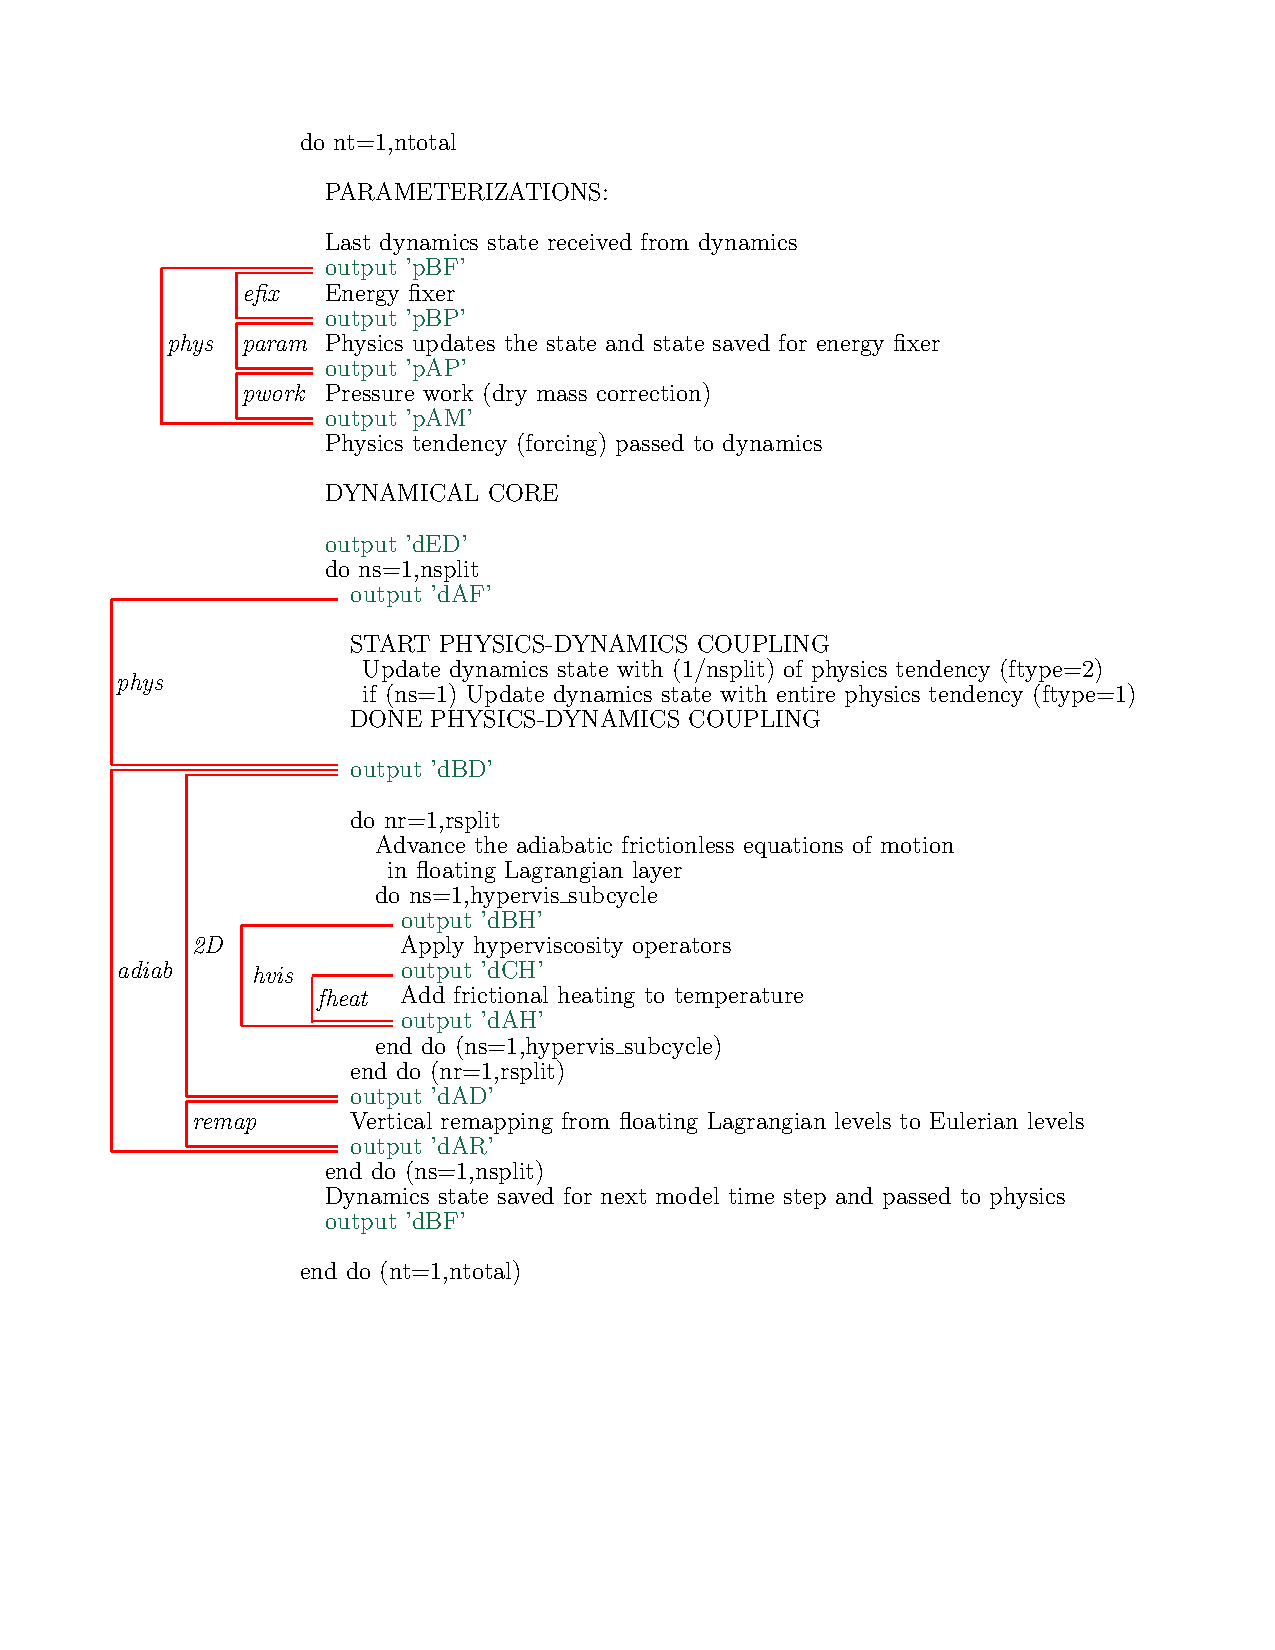
\includegraphics[width=35pc]{new_pseudo-code.pdf}
\caption{Pseudo-code for CAM-SE showing the order in which relevant physics updates are performed as well as dynamical core steps and associated loops. In green font locations where the state is captured and output is shown together with its 3 character identifier. The outer most loop ($1,ntotal$)  advances the entire model $\Delta t_{phys}$ seconds (in this case 1800s). The dynamical core loops are as follows: the outer loop is the vertical remapping loop (1,{\tt{nsplit}}) with associated time-step $\Delta t_{phys}/{\tt{nsplit}}$. For stability the temporal advancement of the equations of motion in the Lagrangian layer needs to be sub-cycled {\tt{rsplit}} times. Within the {\tt{rsplit}}-loop the hyperviscosity time-stepping is sub-cycled $hypervis\_subcycle$ times (again for stability). For more details on the time-stepping in CAM-SE see \citet{LetAl2018JAMES}.}
\label{fig:dAD}
\end{figure}


We now define the following energy tendencies corresponding to the itemized list in section \ref{subsec:spuriousE} with references to terms indicated in Figure \ref{fig:dAD}. We start just after the energy fixer which will be defined at the end.
\begin{enumerate}
%
\item $\partial \gi{E}^{(param)}$: TE tendency due to parameterizations. In CAM the TE budget for each parameterization is closed (assuming pressure is unchanged) so $\partial \gi{E}^{(param)}$ is balanced by net fluxes in/out of the physics columns. Note that this is the only energy tendency that is not spurious since CAM parameterizations have a closed TE budget. This TE tendency is discretely computed as
\begin{equation}
\partial \gi{E}_{phys}^{({param})}=\frac{\gi{E}_{pAP}-\gi{E}_{pBP}}{\Delta t_{phys}},
\end{equation}
where $\Delta t_{phys}$ is the physics time-step (default 1800s) and the subscript $phys$ on $\partial \gi{E}$ refers to the energy tendency computed in CAM physics. 
%
\item $\partial \gi{E}^{({pwork})}$: Total spurious energy tendency due to pressure work {\color{red}{error}}
\begin{equation}
\partial \gi{E}_{phys}^{({pwork})}=\frac{\gi{E}_{pAM}-\gi{E}_{pAP}}{\Delta t_{phys}}.
\end{equation}
Since CAM-SE dynamical core is based on a dry-mass vertical coordinate the pressure work {\color{red}{error}} takes place implicitly in the dynamical core. But the TE tendency due to pressure work {\color{red}{error}} is conveniently computed in physics since dynamical cores based on a moist vertical coordinate (e.g., CAM-FV) require pressure and moist mixing ratios to be adjusted for dry mass conservation and tracer mass conservation \citep[section 3.1.8 in ][]{CAM5}. The difference of TE after and before this adjustment is the TE tendency due to pressure work {\color{red}{error}}. In a dry mass vertical coordinate based on dry mixing ratios neither dry mass layer thickness nor dry mixing ratios need to be adjusted to take into account moisture changes in the column. For labeling purposes, the 'total forcing' associated with physics (at least in CAM) consists of parameterizations, pressure work {\color{red}{error}} and TE fixer, although strictly speaking the fixer includes components from the dynamics as will be seen.
\begin{equation}
\partial \gi{E}_{phys}^{({phys})}\equiv \partial \gi{E}_{phys}^{({param})}+\partial \gi{E}_{phys}^{({pwork})}+\partial \gi{E}_{phys}^{({efix})}=\frac{\gi{E}_{pAM}-\gi{E}_{pBF}}{\Delta t_{phys}}.
\end{equation}
where the energy fixer TE tendency is
\begin{equation}
\partial \gi{E}_{phys}^{({efix})}=\frac{\gi{E}_{pBP}-\gi{E}_{pBF}}{\Delta t_{phys}}.
\label{efix.def}
\end{equation}
After all the TE budget terms have been defined, the exact composition of $\partial \gi{E}_{phys}^{({efix})}$ will be presented.

\item $\partial \gi{E}^{({discr})}$: If the physics uses a TE definition different from the TE that the continuous equations of motion in the dynamical core conserve (i.e. in the absence of discretization errors), then there is a TE discrepancy tendency. This complicates the energy analysis as one can not compare TE computed in physics $\gi{E}_{phys}$ directly with TE computed in the dynamical core $\gi{E}_{dyn}$. This makes errors associated with this discrepancy tricky to assess. That said, the TE tendencies computed using the dynamical core TE formula $\partial \gi{E}_{dyn}$ are well defined (self consistent) and similarly for TE tendencies computed using the `physics formula' for TE, $\partial \gi{E}_{phys}$.


\item The TE tendency from the dynamical core is split into several terms:
Horizontal adiabatic dynamics (dynamics excluding physics forcing tendency)
\begin{equation}
\partial \gi{E}_{dyn}^{({2D})}=\frac{\gi{E}_{dAD}-\gi{E}_{dBD}}{\Delta t_{dyn}},
\end{equation}
where over a single dynamics sub-step $\Delta t_{dyn}=\frac{\Delta t_{phys}}{{\tt{nsplit}}\times {\tt{rsplit}}}$ (the loop bounds {\tt{nsplit}}, {\tt{rsplit}}, etc. are explained in Figure \ref{fig:dAD}).

In CAM-SE the viscosity is explicit so one can compute the TE tendency due to hyperviscosity and its associated frictional heating
\begin{equation}
\partial \gi{E}_{dyn}^{({hvis})}=\frac{\gi{E}_{dAH}-\gi{E}_{dBH}}{\Delta t_{hvis}},
\end{equation}
which, in CAM-SE, includes a frictional heating term from viscosity on momentum
\begin{equation}
\partial \gi{E}_{dyn}^{({fheat})}=\frac{\gi{E}_{dAH}-\gi{E}_{dCH}}{\Delta t_{hvis}},
\end{equation}
where $\Delta t_{hvis}=\frac{\Delta t_{phys}}{{\tt{nsplit}}\times {\tt{rsplit}} \times hypervis\_subcycle}$ is the time step of the sub-stepped viscosity. The residual
\begin{equation}
\partial \gi{E}_{dyn}^{(res)}=\partial \gi{E}_{dyn}^{({2D})}-\partial \gi{E}_{dyn}^{({hvis})},
\end{equation}
is the energy error due to inviscid dynamics and time-truncation errors.

The energy tendency due to vertical remapping is
\begin{equation}
\partial \gi{E}_{dyn}^{({remap})}=\frac{\gi{E}_{dAR}-\gi{E}_{dAD}}{\Delta t_{remap}},
\end{equation}
where $\Delta t_{remap}=\frac{\Delta t_{phys}}{{\tt{nsplit}}}$.

The 3D adiabatic dynamical core (no physics forcing but including friction) energy tendency is denoted
\begin{equation}
\partial \gi{E}_{dyn}^{({adiab})}=\partial \gi{E}_{dyn}^{({2D})}+\partial \gi{E}_{dyn}^{({remap})}.
\end{equation}

\item $\partial \gi{E}^{(pdc)}$: Total spurious energy tendency due to physics-dynamics coupling errors is the difference between the energy tendency from physics and the energy tendency in the dynamics resulting from adding the physics increment to the dynamical core state
\begin{equation}
  \label{eq:pdc}
\partial \gi{E}^{(pdc)}=\partial \gi{E}_{phys}^{({phys})}-\partial \gi{E}_{dyn}^{({phys})} \text{ assuming }\partial \gi{E}^{({discr})}=0,
\end{equation}
where
\begin{equation}
\partial \gi{E}_{dyn}^{({phys})}=\frac{\gi{E}_{dBD}-\gi{E}_{dAF}}{\Delta t_{pdc}},
\end{equation}
and $\Delta t_{pdc}$ is the time-step between physics increments being added to the dynamical core. Remember we are dealing with average rates so terms computed with different time steps can be compared, but differences cannot be taken between terms sampled with different time steps.

The physics-dynamics coupling TE tendency $\partial \gi{E}^{(pdc)}$ makes use of TE formulas in dynamics and in physics so \eqref{eq:pdc} is only well-defined if the TE formula discrepancy is zero, $\partial \gi{E}^{({discr})}=0$. As mentioned in Section \ref{sec:defE}, CAM-SE has the option to switch the continuous equations of motion conserving the TE used by CAM physics \eqref{eq:Ephys} instead of the more comprehensive TE formula \eqref{eq:comprehensice_energy}.

In CAM-SE there are 3 physics-dynamics coupling algorithms described in detail in section 3.6 in \citet{LetAl2018JAMES} and reviewed in the introduction here. One is {\em{state-update}} in which the entire physics increments are added to the dynamics state at the beginning of dynamics (referred to as {\tt{ftype=1}}), in which case $\Delta t_{pdc}=\Delta t_{phys}$. Another is {\em{dribbling}} in which the physics tendency is split into {\tt{nsplit}} equal chunks and added throughout dynamics (more precisely after every vertical remapping; referred to as {\tt{ftype=0}} resulting in $\Delta t_{pdc}=\frac{1}{{\tt{nsplit}}}\Delta t_{phys}$), and then a {\em{combination}} of the two (referred to as {\tt{ftype=2}}) where tracers (mass variables) use {\em{state-update}} ({\tt{ftype=1}}) and all other physics tendencies use {\em{dribbling}} ({\tt{ftype=0}}). 
%The various parameters for defining time-steps in terms of `split parameters' (such as {\tt{nsplit}}) are defined in Figure \ref{fig:dAD}.
%where the subscript $phys$ in $\partial \gi{E}_{phys}^{({phys})}$ refers to the TE tenendency being computed in CAM physics using the formula for energy consistent with physics \eqref{eq:Ephys}. In CAM the vertical and horizontal grids in physics and dynamics coincide  so physics-dynamics coupling errors are due to the temporal aspect of coupling (errors due to `dribbling' tendencies in the dynamical core). The TE tenendency due to physics tendencies being added to the dynamical core is
%\begin{equation}
%\partial \gi{E}^{({phys})}_{dyn}=
%\end{equation}
%If the same energy definition is used in the physics and dynamical core, and an energy conservative physics dynamics coupling method is used, then $\partial \gi{E}_{phys}^{({param})}$.

\item $\partial \gi{E}^{({efix})}$: Global energy fixer tendency, defined in \eqref{efix.def}, is applied at the beginning of the parameterizations. The correction needed is the global average difference between the state passed from the dynamics and the state that was saved after the physics updated the state  but before the dry mass correction. It includes all spurious sources from the dry mass correction, remappings between physics and dynamics, dynamical core, differing energy definitions (if present), hyperviscosity, and vertical remapping.

\end{enumerate}

\subsection{A few observations regarding the energy budget terms}
It is useful to note that the energy fixer `fixes' energy errors for the dynamical core, pressure work {\color{red}{error}}, physics-dynamics coupling and TE discrepancy
\begin{equation}
\label{eq:budget_efix}
-\partial \gi{E}_{phys}^{({efix})}=\partial \gi{E}_{phys}^{({pwork})}+\partial \gi{E}_{dyn}^{({adiab})}+\partial \gi{E}^{({pdc})}+\partial \gi{E}^{({discr})}.
\end{equation}
The forcing from the parameterizations, $\partial \gi{E}_{phys}^{({param})}$, does not appear in this budget (although the dynamical core state does `feel' the parameterization forcing) as the energy cycle for the parameterizations is, by design in CAM, closed (balanced by fluxes in/out of the physics columns). If $\partial \gi{E}^{({discr})}=0$, one can use \eqref{eq:budget_efix} to diagnose energy dissipation in the dynamical core and physics-dynamics coupling from quantities computed only in physics
\begin{equation}
\label{eq:pdc2}
\partial \gi{E}_{dyn}^{({adiab})}+\partial \gi{E}^{({pdc})}=-\partial \gi{E}_{phys}^{({efix})}-\partial \gi{E}_{phys}^{({pwork})} \text{ for  }\partial \gi{E}^{({discr})}=0.
\end{equation}
This is useful if the diagnostics are not implemented in the dynamical core; in particular, if the {\em{state-update}} ({\tt{ftype=1}}) physics-dynamics coupling method is used then $\partial \gi{E}^{({pdc})}=0$ and the TE errors in the dynamical core can be computed without diagnostics implemented in the dynamical core. Also, \eqref{eq:pdc2} provides an alternative formula for $\partial \gi{E}^{({pdc})}$ compared to \eqref{eq:pdc}:
\begin{equation}
\label{eq:pdc3}
\partial \gi{E}^{({pdc})}=-\partial \gi{E}_{phys}^{({efix})}-\partial \gi{E}_{phys}^{({pwork})}-\partial \gi{E}_{dyn}^{({adiab})} \text{ assuming }\partial \gi{E}^{({discr})}=0.
\end{equation}
If $\partial \gi{E}^{({pdc})}=0$ \eqref{eq:budget_efix} can be used to compute $\partial \gi{E}^{({discr})}$
\begin{equation}
\label{eq:discre}
\partial \gi{E}^{({discr})}=-\partial \gi{E}_{phys}^{({efix})}-\partial \gi{E}_{phys}^{({pwork})}-\partial \gi{E}_{dyn}^{({adiab})}, \text{ assuming }\partial \gi{E}^{(pdc)}=0.
\end{equation}
Note that we can not use \eqref{eq:pdc} to compute $\partial \gi{E}^{({discr})}$ since $\gi{E}_{phys}\neq \gi{E}_{dyn}$.
%
\begin{sidewaystable}
  \caption{TE tendencies in units of $W/m^2$ associated with various aspects of CAM-SE run in AMIP-type setup (unless otherwise noted). Column 1 is the identifier for the model configuration. See the text for a brief summary of these descriptors. They are defined in more detail in the following sections where the section titles also include the `Descriptor' from Table \ref{table:TE} to make it easier for the reader to match Table entries with discussion in the text. Column 2 is $\mathcal{N}=${\tt{qsize\_condensate\_loading}} identifying how many water species are thermodynamically{\color{red}{/inertially}} active in the dynamical core (see section \ref{sec:defE} for details). Column 3, {\tt{lcp\_moist}}, indicates whether or not the heat capacity includes water variables or not and column 4 shows physics-dynamics coupling method {\tt{ftype}}. The TE tendencies $\partial \gi{E}$ in columns 5-14 are defined in section \ref{sec:diagnostics}. If $\partial \gi{E}$ is less than $10^{-5}$ $W/m^2$ it is set to zero in the Table. Significant changes compared to the baseline ({\em{TE consistent}} configuration) discussed in the main text are in bold font.}
\label{table:TE}
\begin{tabular}{c|ccc|ccc|cccccc|c}
Descriptor & $\mathcal{N}$ & {\tt{lcp\_moist}} &  {\tt{ftype}}  & $\partial \gi{E}_{phys}^{({pwork})}$ &  $\partial \gi{E}_{phys}^{({efix})}$ &  $\partial \gi{E}_{phys}^{({discr})}$ &  $\partial \gi{E}_{dyn}^{({2D})}$ & $\partial \gi{E}_{dyn}^{({hvis})}$ & $\partial \gi{E}_{dyn}^{({fheat})}$ & $\partial \gi{E}_{dyn}^{(res)}$ & $\partial \gi{E}_{dyn}^{(remap)}$ & $\partial \gi{E}_{dyn}^{(adiab)}$  & $\partial \gi{E}^{(pdc)}$\\
\hline \hline \\
% %5 year average
{\em{TE consistent}}& 1 & false & 1 &  0.312&  0.300& 0    & -0.601& -0.608&  0.565& 0.007          & -0.011& -0.613 &  0\\
{\em{`dribbling' A}}& 1 & false & 0 &  0.315&  0.313& 0    & -0.577& -0.584&  0.568& 0.007          & -0.011& -0.588 &  {\bf{0.469}}\\
{\em{`dribbling' B}}& 1 & false & 2 &  0.316&  0.341& 0    & -0.598& -0.606&  0.563& 0.008          & -0.011& -0.609 &  {\bf{0.484}}\\
{\em{vert limiter}} & 1 & false & 1 &  0.317&  0.472& 0    & -0.590& -0.597&  0.509& 0.006          & {\bf{-0.199}} & -0.789 &  0\\
%
% adiabtic dycore becomes source of energy
%
%{\em{no patc}}     & 1 & false & 1 &  0.309& -0.737& 0    &  0.439&  0.429&  0.604& 0.0106           & -0.011& 0.428& 1.03e-07\\
%{\em{HOMME}}       & 1 & false & 1 &  0.304&   -0.4& 0    &  0.103&  0.095&  0.754& 0.00753          & -0.007& 0.095& -3.44e-08\\
%
% smoother topography
%
{\em{smooth topo}} & 1 & false & 1  &  0.315& {\bf{-0.008}}& 0  & {\bf{-0.295}}& {\bf{-0.300}}  &  0.493& 0.005          & -0.012& {\bf{-0.307}} & 0\\
{\em{energy discr}} & 5 & true  & 1 &  0.332& -0.313& {\bf{0.594}}& -0.603& -0.612&  0.575& 0.009          & -0.011& -0.614 & -\\
{\em{default}}      & 5 & true  & 2 &  0.316& -0.272&             & -0.578& -0.587&  0.579& 0.010          & -0.012& -0.589 & -\\ %23 years
%{\em{default}}      & 5 & true  & 2 &  0.316& -0.272& {\bf{0.546}}& -0.578& -0.587&  0.579& 0.010          & -0.012& -0.589 & -\\ %23 years
\hline
{\em{QPC6}}         & 1 & false & 1 &  0.305& -0.169& 0    &{\bf{-0.129}}& {\bf{-0.131}}&  0.477& 0.001 & -0.007& {\bf{-0.136}} & 0\\
{\em{FHS94}}        & 1 & false & 2 &  -    &   -   &  -   & {\bf{-0.025}}&{\bf{-0.025}} &  0.122& 0 &  0.005 & {\bf{-0.020}} & -\\
{\em{FV}}       & 1 & false & 1 &  0.304&  0.670& 0    & - & - & - & - & - & {\bf{-0.974}} & 0 \\
{\em{CSLAM}} & 1 & false & 1 &  0.312& 0.239& 0 & -0.547& -0.557&   0.620&   0.010& -0.011& -0.558& {\bf{-0.070}}\\
{\em{CSLAM default}} & 5 & true   & 2   &   0.320& -0.342&  - & -0.524& -0.537&  0.641& 0.013& -0.011& -0.535& - 
  \end{tabular}
  \end{sidewaystable}

\section{Results}
\label{sec:results}
A series of simulations have been performed with CESM2.1 using CAM version 6 (CAM6) physics (\url{https://doi.org/10.5065/D67H1H0V}) on NCAR's Cheyenne cluster \citep{cheyenne}. All simulations are at nominally $\sim1^{\circ}$ horizontal resolution (for CAM-SE that is 30$\times$30 elements on each cubed-sphere face and for CAM-FV its 192$\times$288 latitudes-longitudes) and using the standard 32 levels in the vertical. Unless otherwise noted all simulations are 13 months in duration and the last 12 months are used in the analysis. Total energy budgets are summarized in Table \ref{table:TE} and discussed below. The first column gives identifying `Descriptors' which are briefly summarized below and defined in more detail in the following sections. The section titles also include the `Descriptor' from Table \ref{table:TE} to make it easier for the reader to match Table entries with discussion in the text. Important changes to TE errors are marked with bold font in Table \ref{table:TE}.

Various configurations are used and referred to in terms of the $COMPSET$ (Component Set) value used in CESM2.1 The $COMPSET$ {\em{F2000climo}} configuration refers to `real-world' AMIP (Atmospheric Model Intercomparison Project) type simulations using perpetual year 2000 SST (Sea Surface Temperature) boundary conditions. The first 7 simulations in the table (those above the horizontal line) are such AMIP-type simulations (F2000climo) with the first serving as a control for the 6 following variants. The remaining 5 simulation descriptors (below the horizontal line in Table \ref{table:TE}) list their $COMPSET$ or dynamical core settings.

\begin{itemize}
\item {\em{TE consistent}}: The TE consistent version uses {\em{state update}} physics-dynamics coupling ({\tt{ftype 1}}) described in section \ref{sec:consistent},
\item {\em{`dribbling' A}}: as {\em{TE consistent}} but with {\em{dribbling}} physics-dynamics coupling ({\tt{ftype 0}}) (section \ref{se:pdc_problem}),
\item {\em{`dribbling' B}}: as {\em{TE consistent}} but with  {\em{dribbling}} combination physics-dynamics coupling ({\tt{ftype 2}}) (section \ref{se:pdc_problem}),
\item {\em{vert limiter}}: as {\em{TE consistent}} but using limiters in the vertical remapping of momentum (section \ref{sec:ppm}),
\item {\em{smooth topo}}: as {\em{TE consistent}} but  using smoother topography (see section \ref{sec:topo}),
\item {\em{energy discr}}: The version with energy discrepancy (but no physics-dynamics coupling errors) described in section \ref{sec:ediscr},
\item {\em{default}}: as {\em{energy discr}} version but with {\tt{ftype=2}} which is the current default CAM-SE (section \ref{sec:ediscr}),
\item {\em{QPC6}}: A simplified aqua-planet setup based on the {\em{TE consistent}}, i.e an aqua-planet setup using CAM6 physics; an ocean covered planet in perpetual equinox, with fixed, zonally symmetric sea surface temperatures \citep{NH2000ASL,MWO2016JAMES} (section \ref{sec:QPC6}), 
\item {\em{FSH94}}: Dry dynamical core configuration based on Held-Suarez forcing which relaxes temperature to a zonally symmetric equilibrium temperature profile and simple linear drag at the lower boundary \citep{HS1994BAMS} (section \ref{sec:FHS94}),. 
\item {\em{FV}}: A configuration with the SE dynamical core replaced with the finite-volume core (section \ref{sec:cam-fv}), and
\item {\em{CSLAM}}: The quasi equal-area physics grid configuration of CAM-SE based on the TE consistent setup (section \ref{sec:cslam})
\item {\em{CSLAM default}}: Same as {\em{CSLAM}} configuration but with {\tt{ftype=2}} and all forms of water thermodynamically{\color{red}{/inertially}} active in the dynamical core.
\end{itemize}


 \begin{figure}[h]
 \centering
 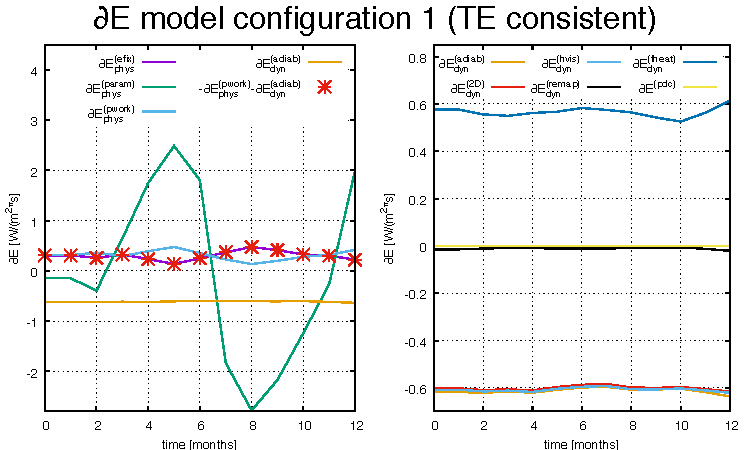
\includegraphics[width=35pc]{dEdt.pdf}
 \caption{Monthly averaged TE tendencies as a function of time for various aspects of the TE consistent configuration of CAM-SE run in AMIP-type configuration with perpetual year 2000 SSTs. Left Figure shows $\partial \gi{E}$ TE tendencies in physics and, for comparison, TE tendency for the adiabatic dynamical core. The right plot shows the break-down of $\partial \gi{E}$ for the dynamical core. These plots show that the energy tendency from the dynamical core is quite constant (to within $\sim 0.02W/m^2$ or less) so only one month simulations is adequate to assess energy diagnostics for the dynamical core. For more details see Section \ref{sec:consistent}.}
 \label{fig:dEdt(t)}
  \end{figure}




\subsection{{\em{TE consistent}}: {\em{state-update}} physics-dynamics coupling ({\tt{ftype=1}}) and no TE formula discrepancy}
\label{sec:consistent}
This configuration is the most energetically consistent in that the physical parameterizations and the continuous equations of motion on which the dynamical core is based, conserve the same TE (defined in equation \eqref{eq:Ephys}); and there are no spurious sources/sinks in physics-dynamics coupling. Energetic consistency in dynamics and physics is obtained by setting $c_p^{(\ell)}\equiv c_p^{d}$ and $\mathcal{L}_{all}=\left\{ `d`,`wv`\right\}$ in the dynamical core equations of motion and TE computations. Associated namelist changes resulting in this configuration are $\tt{lcp\_moist=.false.}$, $\tt{se\_qsize\_condensate\_loading=1}$, and $\tt{ftype=1}$. 
%If the parameterizations effectively update the model state then there are no physics-dynamics coupling errors \citep[$\tt{ftype=1}$ setup described in detail in ][]{LetAl2018JAMES}. 

The TE consistent configuration in AMIP-type simulation ({\em{F2000climo}}) is used to compute baseline TE tendencies which will be used to compare with other model configurations. First we establish how long an average is needed to get robust TE tendency estimates. Figure \ref{fig:dEdt(t)} shows $\partial \gi{E}$ for various aspects of CAM-SE as a function of time. The simulation length is 5 years and monthly average values are used for the analysis. First consider the left plot. The TE tendency from parameterizations ($\partial \gi{E}^{(param)}_{phys}$) show significant variability with an amplitude of approximately 2.5$W/m^2$. As noted above this term does not figure in the spurious TE budget. The net source/sink provides an equal and opposite term to balance it. That said, the variability is reflected onto the TE tendency due to pressure work {\color{red}{error}} $\partial \gi{E}^{(pwork)}_{phys}\approx 0.32\pm 0.08 W/m^2$. On the scale used in the left-hand plot the TE tendency of the adiabatic dynamical core $\partial \gi{E}^{(adiab)}_{dyn}$ does not seem to be affected by $\partial \gi{E}^{(param)}_{phys}$ or $\partial \gi{E}^{(pwork)}_{phys}$ in terms of variability, and remains stable at approximately -0.6$W/m^2\pm ~0.02 W/m^2$. The TE fixer, in this model configuration, fixes $\partial \gi{E}^{(adiab)}_{dyn}$ and $\partial \gi{E}^{(pwork)}_{phys}$. Since the TE imbalance in the adiabatic dynamics remains approximately constant and the TE tendency associated with pressure work {\color{red}{error}} has variability, the TE tendency from the $\partial \gi{E}^{(efix)}_{phys}$ has variability; $\partial \gi{E}^{(efix)}_{phys}\approx 0.30 \pm 0.08 W/m^2$. As a consistency check $-\partial \gi{E}^{(adiab)}_{dyn}-\partial \gi{E}^{(pwork)}_{phys}$ is plotted with asterisk's and they coincide (as expected) with $\partial \gi{E}^{(efix)}_{phys}$ fulfilling \eqref{eq:budget_efix}.

The right-hand plot in  Figure \ref{fig:dEdt(t)} shows a breakdown of the dynamical core TE tendencies. The majority of the TE errors are due to hyperviscosity on temperature and pressure, $\partial \gi{E}^{(hvis)}_{dyn}\approx -0.61\pm 0.01 W/m^2$. The diffusion of momentum is added back as frictional heating and is therefore not part of $\partial \gi{E}^{(hvis)}_{dyn}$. The frictional heating is a significant term in the TE tendency budget $\partial \gi{E}^{(fheat)}_{dyn}\approx 0.56\pm 0.02 W/m^2$ and exhibits some variability but with a rather small amplitude. The remaining TE error in the floating Lagrangian dynamics is inviscid dissipation and time-truncation errors $\partial \gi{E}_{dyn}^{(res)}=\partial \gi{E}_{dyn}^{({2D})}-\partial \gi{E}_{dyn}^{({hvis})}\approx 0.007 W/m^2$. The TE tendency from vertical remapping is approximately $\partial \gi{E}_{dyn}^{({remap})}\approx -0.01 W/m^2$. To within $\sim 0.02 W/m^2$ the dynamical core TE tendency terms can be computed from just one month average TE integrals. The TE tendencies computed in physics, excluding $\partial \gi{E}^{(param)}_{phys}$, exhibit more variability and are only accurate to $\sim 0.1 W/m^2$ after a one month average.

While it is advantageous to use {\em{state-update}} physics-dynamics coupling algorithm ({\tt{ftype=1}}) in terms of having no spurious TE tendency from coupling, $\partial \gi{E}^{({pdc})}=0$, it does result in spurious gravity waves in the simulations \cite[see, e.g., Figure 5 in ][]{GetAl2018MWR}. Figure \ref{fig:abs_dpsdt}a shows a 1 year average of $|\frac{dp_s}{dt}|$, a measure of high frequency gravity wave noise. It clearly exhibits unphysical oscillations coinciding with element boundaries. Details of the spectral-element method, its coupling to physics and associated noise issues are discussed in detail in \citet{HetAl2018MWR}. The noise in the solutions is even visible in the 500hPa pressure velocity annual average (Figure \ref{fig:omega500}a). This issue can be alleviated by using a shorter physics time-step so that the physics increments are smaller (not shown). Climate modelers have historically not pursued a shorter physics time-step in production configurations as climate parameterizations are computationally expensive and there is a large sensitivity to physics time-steps in the simulated climate \citep[e.g.][]{WO2003QJR,WetAl2015JAMES}.

\subsection{{\em{`dribbling' A/B}}: Non-TE conservative physics-dynamics coupling ({\tt{ftype=0,2}})}\label{se:pdc_problem}
{\color{red}{Before discussing the impact of different PDC methods on the TE budget, we discuss element boundary noise issues in CAM-SE which are related to PDC method. This motivates the different PDC methods implemented in CAM-SE.}}
\subsubsection{{\color{red}{Spurious }}element boundary noise {\color{red}{from physics-dynamics coupling}}}\label{sec:noise}
When switching to {\em{dribbling}} physics-dynamics coupling algorithm ({\tt{ftype=0}}) in which the tendencies from physics are added throughout the dynamics (in this case twice per physics time-step) then the noise issues described in previous section disappear (Figure \ref{fig:abs_dpsdt}b and \ref{fig:omega500}b). That said, there is a significant issue with this approach; the tracer mass budgets may not be closed. How this comes about is illustrated in Figure \ref{fig:ftype_schematic} and explained in the next paragraph. 

The orange curve on Figure \ref{fig:ftype_schematic}a, b, d, and e is the initial state of, e.g., cloud liquid mixing ratio as a function of location, e.g., longitude. Cloud liquid is zero outside of clouds and hence provides a good example for the purpose of this illustration. The light blue arrows show the increments (in terms of length of arrow) computed by the parameterizations based on the initial state and scaled for the partial update with {\em{dribbling}} ({\tt{ftype=0}}). With {\em{state-update}} ({\tt{ftype=1}}) the increments from physics are added to the dynamical core state (dotted line on \ref{fig:ftype_schematic}b) before the dynamical core advances the solution in time. The parameterizations are designed to not drive the mixing ratios negative so the state-update in dynamics will not generate negatives (or overshoots). Then the dynamical core advects the distribution (solid curve on Figure \ref{fig:ftype_schematic}c). With {\em{dribbling}} ({\tt{ftype=0}}) the physics increments are split into equal chunks (in this illustration two; blue errors on Figure \ref{fig:ftype_schematic}d). Half of the physics increments are added to the initial state (dotted line on Figure \ref{fig:ftype_schematic}e) and then dynamics advects the distribution half of the total dynamical core steps (dashed line on Figure \ref{fig:ftype_schematic}e). Then the other half of the physics increments are applied (in the same location as they were computed by physics). Now after the previous/first advection step the cloud liquid distribution has moved and the mixing ratio may be zero (or less than the increment prescribed by physics) where the physics forcing is applied (e.g., left side of dashed curve). Hence the physics increment is driving the mixing ratios negative in those locations. Thereafter the distribution is advected (solid curve on Figure \ref{fig:ftype_schematic}f). In CAM the increments added in the dynamical core are limited so that they drive the mixing to zero (but not negative) if this problem occurs. This leads to a net source of mass compared to the mass change that the parameterizations prescribe (see Figure \ref{fig:pdc}). Although the average source of mass is small each time-step it always has the same sign (i.e. it is a bias) and therefore accumulates. \citet{water-leak} estimated that this spurious source of mass is equivalent to $\sim 10cm$ sea-level rise per decade in coupled climate simulation experiments.

The majority of the noise with {\em{state-update}} ({\tt{ftype=1}}) physics-dynamics coupling method comes from momentum sources/sinks and heating/cooling. A way to alleviate noise problems and, at the same time, close the tracer mass budgets (in physics-dynamics coupling) is to use {\em{state-update}} ({\tt{ftype=1}}) coupling for tracers and {\em{dribbling}} ({\tt{ftype=0}}) coupling for momentum and temperature (referred to as {\em{combination}}, {\tt{ftype=2}}). Figure \ref{fig:abs_dpsdt}c shows the noise diagnostic $|\frac{dp_s}{dt}|$ for {\em{combination}} ({\tt{ftype=2}}) coupling. Figure \ref{fig:abs_dpsdt}c looks very similar to Figure \ref{fig:abs_dpsdt}b but there is some noise near element boundaries. That said, in terms of vertical pressure velocities {\em{combination}} ({\tt{ftype=2}}) and {\em{dribbling}} ({\tt{ftype=0}}) climates are similar in terms of the level of noise (Figure \ref{fig:omega500}b and \ref{fig:omega500}c). The element noise in CAM-SE with {\em{combination}} ({\tt{ftype=2}}) seen in both $|\frac{dp_s}{dt}|$ and 500hPa pressure velocity can be `removed' by using CAM-SE-CSLAM (Figure \ref{fig:abs_dpsdt}d) which uses a quasi equal-area physics grid and CSLAM \cite[Conservative Semi-LAgrangian Multi-tracer; ][]{LNU2010JCP} consistently coupled to the SE method \citep{LTOUNGK2017MWR}. The noise patterns in vertical velocity off the western coast of South America are present in all CAM-SE simulations (and hence not related to physics-dynamics coupling algorithm) are also `removed' by using CAM-SE-CSLAM \citep{HetAl2018MWR}.
\subsubsection{Spurious TE tendencies from physics-dynamics coupling}
When using the same TE formula in the dynamical core and physics the spurious TE tendency from physics-dynamics coupling can be assessed. {\color{red}{As described in item \ref{item:pdc} (Section \ref{subsec:spuriousE}), PDC errors can be attributed to underlying pressure changes during the `dribbling' of temperature and velocity component increments as well as PDC `clipping' errors in the water variables (the process in which `clipping' occurs is described in detail in the previous subsection). The TE error associated with `clipping' PDC error occurs due to the mass-change prescribed by physics consistent with the fluxes in/out of the physics column does not equal the actual mass change applied to the dynamical core state due to `clipping'}}

{\color{red}{For {\tt{ftype=2}} PDC only the increment for temperature and momentum are {\em{dribbled}} whereas tracer mass is state-updated (no `clipping' errors). This results in a spurious PDC TE tendency of $\partial \gi{E}^{({pdc})}=-0.484 W/m^2$. When using {\tt{ftype=0}} PDC also tracer increments are  {\em{dribbled}} (hence there are `clipping' PDC errors) a similar TE tendency results $\partial \gi{E}^{({pdc})}=-0.469 W/m^2$. The difference between the TE PDC tenendency for {\tt{ftype=2}} and {\tt{ftype=0}} provides an estimate of the TE PDC `clipping' error. The `clipping' PDC TE tenendency is very small $~0.015 W/m^2$.}}

%For {\em{dribbling}} ({\tt{ftype=0}}) and {\em{combination}} ({\tt{ftype=2}}) the PDC TE tendency is $\partial \gi{E}^{({pdc})}=-0.05 W/m^2$ and thus rather small compared to the viscosity TE dissipation rates. Since $\partial \gi{E}^{({pdc})}$ are the same (to the second digit) for  {\em{dribbling}} ({\tt{ftype=0}}) and  {\em{combination}} ({\tt{ftype=2}}) it is the momentum and temperature {\em{dribbling}} errors that dominate $\partial \gi{E}^{({pdc})}$ {\color{red}{and not the PDC `clipping' errors}}.


%{\color{red}{This results in a TE error referred to a `clipping' PDC error since the mass-change prescribed by physics consistent with the fluxes in/out of the physics column does not equal the actual mass change applied to the dynamical core state}}

%{\color{red}{$\partial \gi{E}^{(pdc)}$ computed with \eqref{eq:pdc} is $3.709e-09$ and $\partial \gi{E}^{(pdc)}$ computed with \eqref{eq:pdc3} is $1.265e-05$. Why this discrepancy? Can we consider this noise?}} 
\subsection{{\em{vert limiter}}: Limiters on vertical remapping of momentum}\label{sec:ppm}
CAM-SE uses a floating Lagrangian vertical coordinate \citep{S1945JAS,L2004MWR} which requires the remapping of the atmospheric state from floating levels back to reference levels to maintain computational stability and to provide state data consistent with the physics formulation. The mapping algorithm is based on the mass conservative PPM (Piecewise Parabolic Method) with options for shape-preserving limiters. In CAM-SE momentum components and internal energy are used as the variables mapped in the vertical \citep{LetAl2018JAMES} and, contrary to earlier versions of CAM-SE, there is no limiter on the remapping of wind components. If the shape-preserving limiter is used for momentum mapping then the TE dissipation increases by over an order of magnitude from $\sim 0.01W/m^2$ to $\sim 0.2W/m^2$ (Table \ref{table:TE}).
\subsection{{\em{smooth topo}}: Smoother topography}\label{sec:topo}
Topography for CAM is generated using a new version of the software/algorithm described in \cite{LetAl2015GMD} that is available at \url{https://github.com/NCAR/Topo}. The updates to the software includes smoothing algorithms and the computation of sub-grid-scale orientation of topography. 

The default topography in CAM-SE uses the same amount of topography smoothing as CAM-FV (distance weighted smoother applied to the raw topography on $\sim 3$km cubed-sphere grid with a smoothing radius of 180km referred to as $C60$). When the topography is smoother (in this case using $C92$ smoothing, i.e. smoothing radius of approximately 276km) the hyperviscosity operators are less active leading to reduced TE errors, i.e. $\partial \gi{E}^{(hvis)}_{dyn}$ is reduced in half from approximately $-0.6W/m^2$ to $-0.3W/m^2$. The vertical remapping TE error, however, remains approximately the same. Since the pressure work {\color{red}{error}} is approximately $0.3W/m^2$ it almost exactly compensates for the TE tendency from the dynamical core $\partial \gi{E}^{(adiab)}_{dyn}$. Hence if one would only diagnose the TE tendency from the energy fixer one could mistakenly conclude that the model universally  conserves TE when, in fact, there are compensating TE errors in the system. These compensating errors  can only be diagnosed through a careful breakdown of the total TE tendencies.
\subsection{{\em{default}}: TE formula discrepancy errors}\label{sec:ediscr}
To assess the TE errors due to the discrepancy in the energy formula used by dynamics and physics, a simulation using {\em{state-updating}} ({\tt{ftype=1}}, no {\em{`dribbling}} errors) and thermodynamically{\color{red}{/inertially}} active condensates in the dynamical core ($qsize\_condensate\_loading=5$) and consistent/accurate associated heat capacities $c_p^{(\ell)}$ (namelist {\tt{lcp\_moist=.true.}}) has been performed. In this setup the continuous equations of motion in the dynamical core conserve an energy different from physics, and the energy fixer will restore the `physics' version of energy. Despite the dynamical core now using a more comprehensive formula for energy, the TE dissipation terms in the dynamical core are roughly the same as in the energy consistent versions of the model. Using \eqref{eq:discre} we can assess the TE energy discrepancy errors which result in $\sim 0.59W/m^2$. \citet{T2011LNCSEb} found a similar result just from using the more comprehensive formula for heat capacity (based on dry air and water vapor) and not including thermodynamically{\color{red}{/inertially}} active condensates. As noted before this formulation inconsistency is due to the evolutionary nature of CAM development and it is the intention to remove this inconsistency in future versions of the model.

The default version of CAM-SE uses this configuration but with {\em{combination}} ({\tt{ftype=2}}) which has similar TE characteristics (see Table \ref{table:TE}). That said, the physics-dynamics coupling error from {\em{dribbling}} momentum and temperature tendencies and the energy discrepancy errors can not be separated in this configuration:
\begin{equation}
\label{eq:sum}
\partial \gi{E}^{({pdc})}+\partial \gi{E}^{({discr})}=0.546W/m^2,
\end{equation}
using \eqref{eq:budget_efix}. With {\em{state-updating}} ({\tt{ftype=1}}) (i.e. $\partial \gi{E}^{({pdc})}=0$) the energy discrepancy error was 0.594$W/m^2$ and in the energy consistent setup (i.e. $\partial \gi{E}^{({discr})}=0$) but using {\em{dribbling}} ({\tt{ftype=2}}) we got $\partial \gi{E}^{({pdc})}=0.484W/m^2$. So if the physics-dynamics coupling errors and energy discrepancy errors in the different configurations would be additive, one would have expected $\partial \gi{E}^{({pdc})}+\partial \gi{E}^{({discr})}$ to be over $1W/m^2$ which is clearly not the case \eqref{eq:sum}. Again, it must be concluded that there are canceling errors in the system.

%\subsection{Configuration 3: CMIP6 version}
%By only including dry air and water vapor   in $\rho$ and setting $c_p^{(wv)}= c_p^{(d)}$ in the equations of motion, the dynamical core (in the absence of truncation errors) will conserve the energy used in CAM physics.'

%\subsection{Details of hyperviscosity}
%{\color{red}{Note sure if we should add this section: `HOMME' configuration (no reference level subtraction in pressure level thickness damping and increased divergence damping) - in this configuration $\partial \gi{E}^{(adiab)}_{dyn}$ is 0.1$W/m^2$ - dycore is source of TE energy!!!! Solutions are very very noisy over orography so that could be a spurious source of TE i.e. not a `realistic' configuration. If we will use this configuration we should use smoother topography ...}}

\subsection{{\em{QPC6}}: Simplified surface}\label{sec:QPC6}
By running the model in aqua-planet configuration one can assess the effect of simplifying the surface boundary condition. In particular, without topography forcing the dynamical core is not challenged with respect to stationary near-grid-scale forcing. The TE tendency with respect to pressure work {\color{red}{error}} remains the same $\partial \gi{E}_{phys}^{({pwork})}$ as the AMIP-type simulations, however, the adiabatic dynamical core TE tendency reduces to $\partial \gi{E}_{dyn}^{({adiab})}=-0.14 W/m^2$ (approximately a factor 4 reduction). Most of that reduction is due to viscosity $\partial \gi{E}_{dyn}^{(hvis)}=-0.13 W/m^2$. The frictional heating is roughly the same as AMIP $\partial \gi{E}_{dyn}^{(fheat)}=0.48 W/m^2$ as is the vertical remapping  $\partial \gi{E}_{dyn}^{(remap)}=-0.01 W/m^2$. To evaluate the dynamical cores diffusion of TE it is therefore important to asses the model in a configuration with topography as the wave dynamics generated by topography leads to more active diffusion operators.
\subsection{{\em{FHS94}}: Simplified physics (no moisture)}\label{sec:FHS94}
Simplifying the setup even further by replacing the parameterizations with relaxation towards a zonally symmetric temperature profile and simple boundary layer friction (Held-Suarez forcing) as well as excluding moisture, the TE errors in the dynamical core decreases even further to $\sim 0.002W/m^2$ since there is no small scale forcing. Small scales are only created by the nonlinear dynamics and the physics works to damp them. Hyperviscosity is less active leading to significant reductions compared to aqua-planet and `real-world' simulation results. The TE diffusion in vertical remapping reduces by an order of magnitude compared to the aqua-planet simulations ($\sim 0.0005W/m^2$). This further emphasizes that TE diffusion assessment in a simplified setup is not necessarily telling for the dynamical cores performance with moist physics and topography that challenge the dynamical core in terms of strong grid-scale forcing.
\subsection{{\em{FV}}: Changing dynamical core to Finite-Volume (FV)}\label{sec:cam-fv}
As a comparison the TE error characteristics of the CAM-FV dynamical core are assessed. Although the TE diagnostics have not been implemented in the CAM-FV dynamical core, the TE diagnostics in CAM physics are independent of dynamical core and can therefore be activated with CAM-FV. The CAM-FV dynamical core uses {\em{state-update}} physics-dynamics coupling ({\tt{ftype=1}}) ($\partial \gi{E}^{(pdc)}=0$) and the same TE definition as CAM physics ($\partial \gi{E}^{(discr)}=0$). Hence \eqref{eq:pdc2} can be used to compute the TE errors of the CAM-FV dynamical core, $\partial \gi{E}^{(adiab)}_{dyn}\approx -1 W/m^2$. As we do not have the break-down of $\partial \gi{E}^{(adiab)}_{dyn}$ it can not be determined how much of the TE errors are due to the vertical remapping. Furthermore, CAM-FV contains intrinsic dissipation operators (limiters in the flux operators) making it difficult to assess TE sources/sinks due to dissipation. Note that the pressure work {\color{red}{error}} even with a change of dynamical core remains approximately the same as the CAM-SE configurations.
\subsection{{\em{CSLAM}}: Quasi equal-area physics grid}\label{sec:cslam}
This configuration was discussed in the context of element noise in section \ref{sec:noise}. By averaging the dynamics state of an equal-partitioning (in central angle cubed-sphere coordinates) of the elements, the element-boundary noise found in CAM-SE can be removed. \cite{LetAl2018JAMES} argue that this way of computing the state for the physics is more consistent with physics in terms of providing a cell-averaged state instead of irregularly spaced point (quadrature) values. In order to achieve a closed mass-budget, this configuration uses CSLAM for tracer transport rather than SE transport. That said, the physics columns no longer coincide with the quadrature grid and there are TE errors associated with mapping state and tendencies between the two grids.

In this configuration the energy diagnostics computed in the dynamical core are computed on the quadrature grid and the energy diagnostics computed in physics are on the physics grid. If the TE consistent configuration is used ({\tt{ftype=1}}, {\tt{qsize\_condensate\_loading=1}}, {\tt{lcp\_moist=.false.}}) then the physics-dynamical coupling errors, $\gi{E}^{(pdc)}$ computed with \eqref{eq:pdc}, are entirely due to mapping state from quadrature grid to physics grid and mapping tendencies back the quadrature grid from the physics grid. The results is $\gi{E}^{(pdc)}=-0.07W/m^2$ which is a rather small error compared to other terms in the TE budget.

Due to similar noise problems with CAM-SE-CSLAM when using {\tt{ftype=1}} that were observed in CAM-SE (Figure \ref{fig:abs_dpsdt} and \ref{fig:omega500}), the default version of CAM-SE-CSLAM uses {\tt{ftype=2}}. Again physics-dynamics coupling errors and TE discrepancy errors can not be separated; $\partial \gi{E}^{({pdc})}+\partial \gi{E}^{({discr})} = 0.557W/m^2$.

 \begin{sidewaysfigure}
 \centering
 \includegraphics[width=45pc]{abs_dpsdt.pdf}
 \caption{One year average of the absolute surface pressure tendency for (a) the TE consistent configuration, (b) `dribbling' physics-dynamics coupling, (c) {\tt{ftype=2}} physics-dynamics coupling and (d) CSLAM version of CAM-SE, respectively. (a) has a closed physics-dynamics coupling budget but spurious noise, (b) has no spurious noise but the mass-budget in physics-dynamics coupling is not closed (see Figure \ref{fig:pdc}), (c) has a closed mass budget in physics-dynamics coupling but some spurious noise at element boundaries which is eliminated when using CAM-SE-CSLAM (d). Note, the smallest value in panel (a) is the largest in panels (b), (c) and (d).}
 \label{fig:abs_dpsdt}
  \end{sidewaysfigure}


 \begin{sidewaysfigure}
 \centering
 \includegraphics[width=45pc]{omega500.pdf}
 \caption{Same as Figure \ref{fig:abs_dpsdt} but for 500hPa vertical pressure velocity. Note the ringing patterns off the West coast of South America and around the Himalayas in CAM-SE (a-c) that are eliminated with CAM-SE-CSLAM (d) that makes use of a quasi equal-area physics grid.}
 \label{fig:omega500}
  \end{sidewaysfigure}

 \begin{figure}[h]
 \centering
 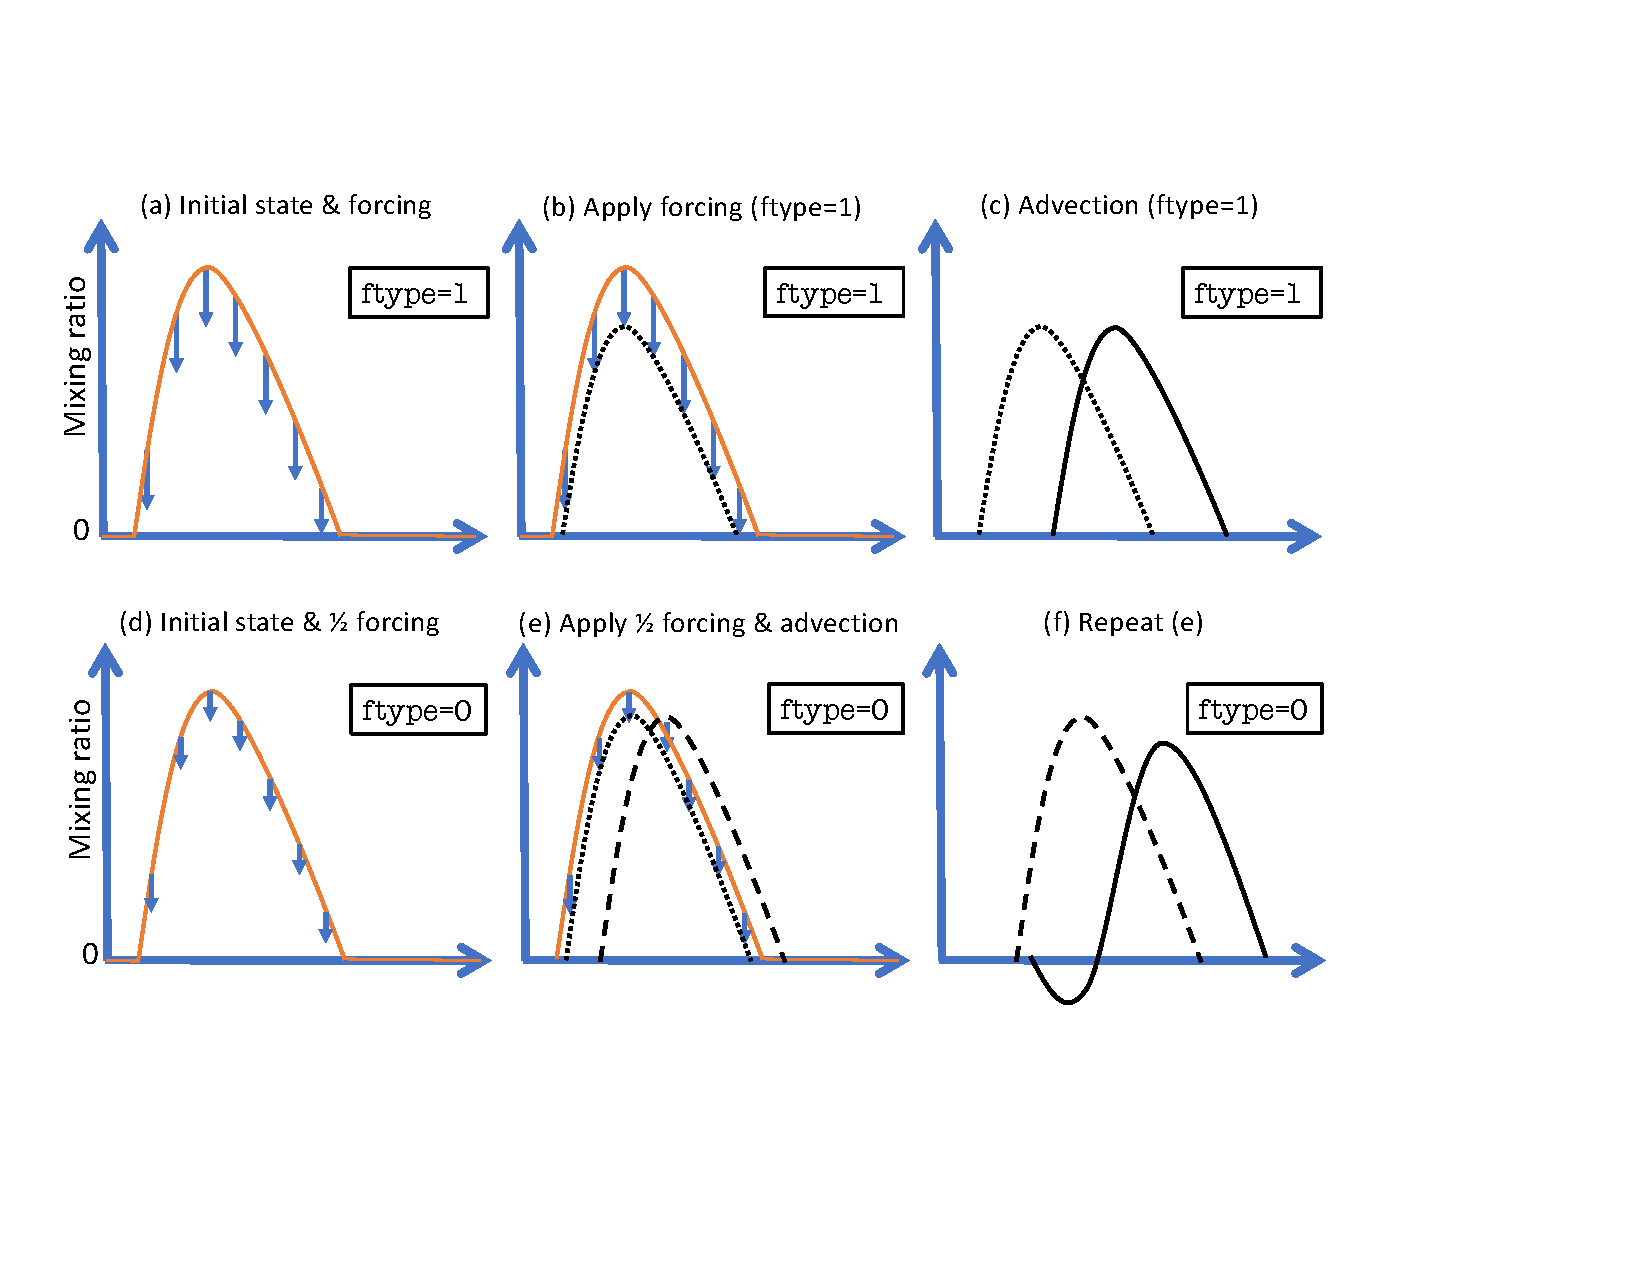
\includegraphics[width=35pc]{ftype_schematic.pdf}
 \caption{A schematic of state-update ({\tt{ftype=1}}; row 1) and `dribbling' ({\tt{ftype=0}}; row 2) physics-dynamics coupling algorithms. See Section \ref{se:pdc_problem} for details.}
 \label{fig:ftype_schematic}
  \end{figure}



 \begin{sidewaysfigure}
 \centering
 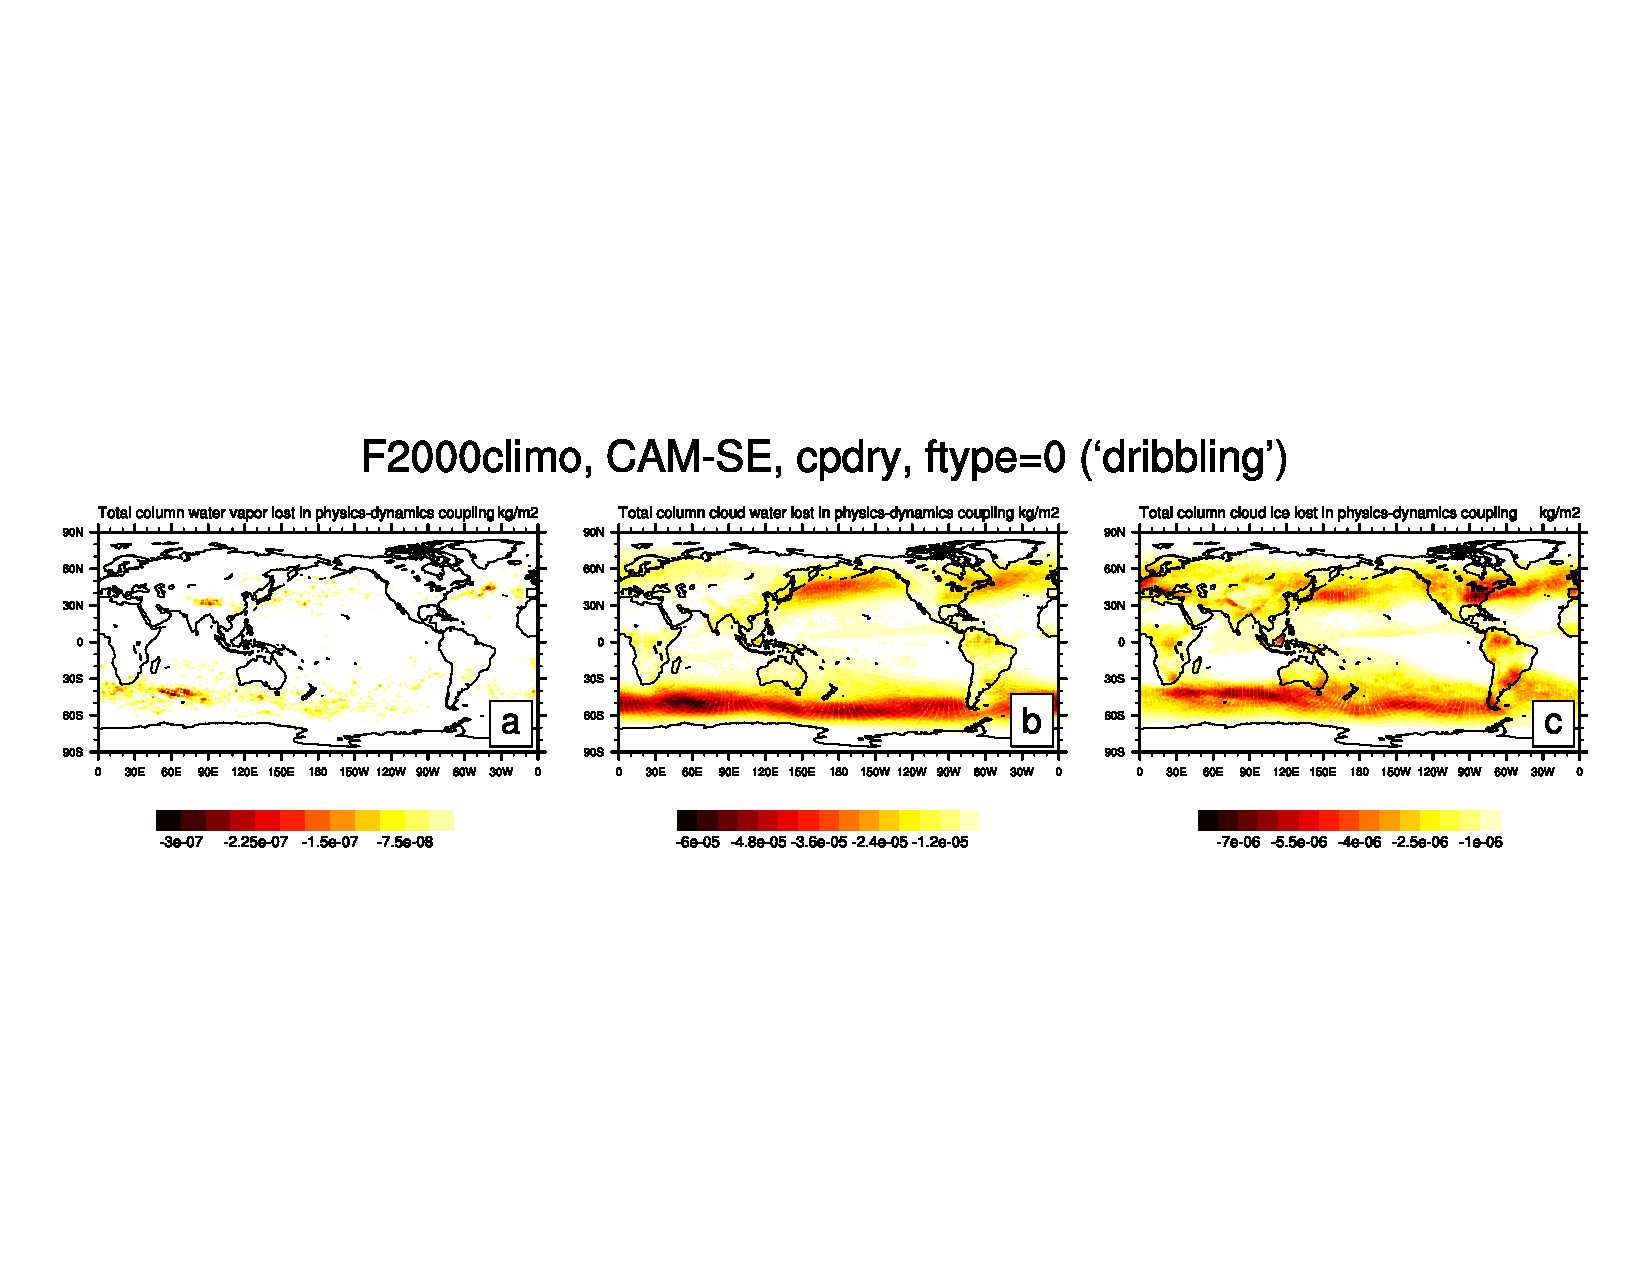
\includegraphics[width=55pc]{pdc.pdf}
 \caption{One year average of mass [$kg/m^2$] `clipped' in physics-dynamics coupling (so that state is not driven negative) when using {\tt{ftype=0}} (`dribbling') physics-dynamics coupling for (a) water vapor, (b) cloud liquid and (c) cloud ice, respectively. Interestingly the element boundaries systematically show in the plots which is likely related to the anisotropy of the quadrature grid \citep{HetAl2018MWR}.}
 \label{fig:pdc}
  \end{sidewaysfigure}


\section{Conclusions}\label{sec:concl}
A detailed total energy (TE) error analysis of the Community Atmosphere Model (CAM) using version 6 physics (included in the CESM2.1 release) running at approximately $1^\circ$ horizontal resolution has been presented. In the global climate model there can be many spurious contributions to the TE budget. These errors can be divided into four categories: physical parameterizations, adiabatic dynamical core, the coupling between physics and dynamics, and TE definition discrepancies between dynamics and physics. The latter is not by design but through the evolutionary nature of model development. By capturing the atmospheric state at various locations in the model algorithm, a detailed budget of TE errors can be constructed. The net spurious TE energy errors are compensated with a global energy fixer (providing a global uniform temperature increment) every physics time-step.

In CAM physics the parameterizations have, by design, a closed energy budget (change in TE is balanced by fluxes in/out the top and bottom of physics columns) if it is assumed that pressure is not modified. However, the pressure changes due to fluxes of mass (e.g., water vapor) in/out of the column which changes energy (referred to as pressure work {\color{red}{error}}). The pressure work {\color{red}{error}} with the full moist physics configuration is very stable across different configurations at $\sim 0.3W/m^2$. The TE errors in the spectral element (SE) dynamical core varies across configurations. Aspects that influence TE is the presence of topography, the amount of topography smoothing and moist physics. By smoothing topography more the TE error is cut in half from $\sim -0.6W/m^2$ to $\sim -0.3W/m^2$; and reduces by a factor of {\color{red}{six}} ($\sim-0.1W/m^2$) if no topography is present at all (aqua-planet configuration). Moist physics forcing also contributes significantly to the TE budget. For example, in the dry Held-Suarez setup TE dissipation of the SE dynamical core reduces to $-0.03W/m^2$. Topography and moist physics force the dynamical core at the grid scale and hence the viscosity operators are more active. Consistent with this statement is that the changes in TE discussed so far are almost entirely due to the viscosity operator TE dissipation. For CAM-SE the spurious TE dissipation in the adiabatic dynamical core is $\sim-0.6W/m^2$ in `real-world' configurations. For comparison, CAM-FV's spurious TE change due to the adiabatic dynamical core is $\sim-1W/m^2$. 

By further breaking down the TE dissipation in the SE dynamical core it is observed the vertical remapping accounts for only $\sim-0.01W/m^2$. That said, if the shape-preserving limiters in the vertical remapping are invoked the TE dissipation increases 20-fold to $\sim-0.2W/m^2$. In CAM-SE the kinetic energy dissipation is added as heating in the thermodynamic equation (also referred to as frictional heating). The frictional heating remains very stable across configurations that include moisture ($\sim 0.5W/m^2$) and reduces drastically for dry atmosphere setups (factor 4 reduction to ($\sim 0.12W/m^2$)). Hence this term is an important term in the TE budget. The TE budget for the dynamical core is dominated by TE change due to hyperviscosity; TE errors due to time-truncation and frictionless equations of motion are negligible. Errors associated with physics-dynamics coupling (if applicable) are approximately $0.5W/m^2$. Due to the evolutionary nature of model development the SE dynamical core's continuous equation of motion conserve a more comprehensive TE compared to the physical parameterizations. This TE discrepancy leads to an approximately $0.5W/m^2$ total energy source. Running physics on a different grid than the dynamical introduces TE mapping errors such as in CAM-SE-CSLAM (Conservative Semi-Lagrangian Multi-tracer transport scheme). These errors are, however, rather small $-0.07W/m^2$.

A purpose of this paper is to better understand the energy characteristics of CAM and to encourage modeling groups to perform similar analysis to better understand the total energy flow in the atmospheric component of Earth system models. As has been demonstrated in this paper there can easily be compensating errors in the system which can not be identified without a detailed TE analysis.

%Text here ===>>>

%%
%  Numbered lines in equations:
%  To add line numbers to lines in equations,
%  \begin{linenomath*}
%  \begin{equation}
%  \end{equation}
%  \end{linenomath*}



%% Enter Figures and Tables near as possible to where they are first mentioned:
%
% DO NOT USE \psfrag or \subfigure commands.
%
% Figure captions go below the figure.
% Table titles go above tables;  other caption information
%  should be placed in last line of the table, using
% \multicolumn2l{$^a$ This is a table note.}
%
%----------------
% EXAMPLE FIGURE
%
% \begin{figure}[h]
% \centering
% when using pdflatex, use pdf file:
% \includegraphics[width=20pc]{figsamp.pdf}
%
% when using dvips, use .eps file:
% \includegraphics[width=20pc]{figsamp.eps}
%
% \caption{Short caption}
% \label{figone}
%  \end{figure}
%
% ---------------
% EXAMPLE TABLE
%
% \begin{table}
% \caption{Time of the Transition Between Phase 1 and Phase 2$^{a}$}
% \centering
% \begin{tabular}{l c}
% \hline
%  Run  & Time (min)  \\
% \hline
%   $l1$  & 260   \\
%   $l2$  & 300   \\
%   $l3$  & 340   \\
%   $h1$  & 270   \\
%   $h2$  & 250   \\
%   $h3$  & 380   \\
%   $r1$  & 370   \\
%   $r2$  & 390   \\
% \hline
% \multicolumn{2}{l}{$^{a}$Footnote text here.}
% \end{tabular}
% \end{table}

%% SIDEWAYS FIGURE and TABLE 
% AGU prefers the use of {sidewaystable} over {landscapetable} as it causes fewer problems.
%
% \begin{sidewaysfigure}
% \includegraphics[width=20pc]{figsamp}
% \caption{caption here}
% \label{newfig}
% \end{sidewaysfigure}
% 
%  \begin{sidewaystable}
%  \caption{Caption here}
% \label{tab:signif_gap_clos}
%  \begin{tabular}{ccc}
% one&two&three\\
% four&five&six
%  \end{tabular}
%  \end{sidewaystable}

%% If using numbered lines, please surround equations with \begin{linenomath*}...\end{linenomath*}
%\begin{linenomath*}
%\begin{equation}
%y|{f} \sim g(m, \sigma),
%\end{equation}
%\end{linenomath*}

%%% End of body of article

%%%%%%%%%%%%%%%%%%%%%%%%%%%%%%%%
%% Optional Appendix goes here
%
% The \appendix command resets counters and redefines section heads
%
% After typing \appendix
%
%\section{Here Is Appendix Title}
% will show
% A: Here Is Appendix Title
%
%\appendix
%   \section{...}

%\section{Here is a sample appendix}

%%%%%%%%%%%%%%%%%%%%%%%%%%%%%%%%%%%%%%%%%%%%%%%%%%%%%%%%%%%%%%%%
%
% Optional Glossary, Notation or Acronym section goes here:
%
%%%%%%%%%%%%%%  
% Glossary is only allowed in Reviews of Geophysics
%  \begin{glossary}
%  \term{Term}
%   Term Definition here
%  \term{Term}
%   Term Definition here
%  \term{Term}
%   Term Definition here
%  \end{glossary}

%
%%%%%%%%%%%%%%
% Acronyms
%   \begin{acronyms}
%   \acro{Acronym}
%   Definition here
%   \acro{EMOS}
%   Ensemble model output statistics 
%   \acro{ECMWF}
%   Centre for Medium-Range Weather Forecasts
%   \end{acronyms}

%
%%%%%%%%%%%%%%
% Notation 
%   \begin{notation}
%   \notation{$a+b$} Notation Definition here
%   \notation{$e=mc^2$} 
%   Equation in German-born physicist Albert Einstein's theory of special
%  relativity that showed that the increased relativistic mass ($m$) of a
%  body comes from the energy of motion of the body—that is, its kinetic
%  energy ($E$)—divided by the speed of light squared ($c^2$).
%   \end{notation}




%%%%%%%%%%%%%%%%%%%%%%%%%%%%%%%%%%%%%%%%%%%%%%%%%%%%%%%%%%%%%%%%
%
%  ACKNOWLEDGMENTS
%
% The acknowledgments must list:
%
% •	All funding sources related to this work from all authors
%
% •	Any real or perceived financial conflicts of interests for any
%	author
%
% •	Other affiliations for any author that may be perceived as
% 	having a conflict of interest with respect to the results of this
% 	paper.
%
% •	A statement that indicates to the reader where the data
% 	supporting the conclusions can be obtained (for example, in the
% 	references, tables, supporting information, and other databases).
%
% It is also the appropriate place to thank colleagues and other contributors. 
% AGU does not normally allow dedications.


\acknowledgments
The National Center for Atmospheric Research is sponsored by the National Science Foundation. Computing resources ({\url{doi:10.5065/D6RX99HX}}) were provided by the Climate Simulation Laboratory at NCAR's Computational and Information Systems Laboratory, sponsored by the National Science Foundation and other agencies. The data used to perform the energy analysis can be found at {\url{https://github.com/PeterHjortLauritzen/2018-JAMES-energy}}.



%% ------------------------------------------------------------------------ %%
%% Citations

% Please use ONLY \citet and \citep for reference citations.
% DO NOT use other cite commands (e.g., \cite, \citeyear, \nocite, \citealp, etc.).


%% Example \citet and \citep:
%  ...as shown by \citet{Boug10}, \citet{Buiz07}, \citet{Fra10},
%  \citet{Ghel00}, and \citet{Leit74}. 

%  ...as shown by \citep{Boug10}, \citep{Buiz07}, \citep{Fra10},
%  \citep{Ghel00, Leit74}. 

%  ...has been shown \citep [e.g.,][]{Boug10,Buiz07,Fra10}.



%%  REFERENCE LIST AND TEXT CITATIONS

\bibliography{bib}
%
% Either type in your references using
%
% \begin{thebibliography}{}
% \bibitem[{\textit{Kobayashi et~al.}}(2003)]{R2013} Kobayashi, T.,
% Tran, A.~H., Nishijo, H., Ono, T., and Matsumoto, G.  (2003).
% Contribution of hippocampal place cell activity to learning and
% formation of goal-directed navigation in rats. \textit{Neuroscience}
% 117, 1025--1035.
%
% \bibitem{}
% Text
% \end{thebibliography}
%
%\bibliography{bib}
%%%%%%%%%%%%%%%%%%%%%%%%%%%%%%%%%%%%%%%%%%%%%%%
% Or, to use BibTeX:
%
% Follow these steps
%
% 1. Type in \bibliography{<name of your .bib file>} 
%    Run LaTeX on your LaTeX file.
%
% 2. Run BiBTeX on your LaTeX file.
%
% 3. Open the new .bbl file containing the reference list and
%   copy all the contents into your LaTeX file here.
%
% 4. Run LaTeX on your new file which will produce the citations.
%
% AGU does not want a .bib or a .bbl file. Please copy in the contents of your .bbl file here.


%% After you run BibTeX, Copy in the contents of the .bbl file here:


%%%%%%%%%%%%%%%%%%%%%%%%%%%%%%%%%%%%%%%%%%%%%%%%%%%%%%%%%%%%%%%%%%%%%
% Track Changes:
% To add words, \added{<word added>}
% To delete words, \deleted{<word deleted>}
% To replace words, \replace{<word to be replaced>}{<replacement word>}
% To explain why change was made: \explain{<explanation>} This will put
% a comment into the right margin.

%%%%%%%%%%%%%%%%%%%%%%%%%%%%%%%%%%%%%%%%%%%%%%%%%%%%%%%%%%%%%%%%%%%%%
% At the end of the document, use \listofchanges, which will list the
% changes and the page and line number where the change was made.

% When final version, \listofchanges will not produce anything,
% \added{<word or words>} word will be printed, \deleted{<word or words} will take away the word,
% \replaced{<delete this word>}{<replace with this word>} will print only the replacement word.
%  In the final version, \explain will not print anything.
%%%%%%%%%%%%%%%%%%%%%%%%%%%%%%%%%%%%%%%%%%%%%%%%%%%%%%%%%%%%%%%%%%%%%

%%%
\listofchanges
%%%

\end{document}

%%%%%%%%%%%%%%%%%%%%%%%%%%%%%%%%%%%%%
%% Supporting Information
%% (Optional) See AGUSuppInfoSamp.tex/pdf for requirements 
%% for Supporting Information.
%%%%%%%%%%%%%%%%%%%%%%%%%%%%%%%%%%%%%



%%%%%%%%%%%%%%%%%%%%%%%%%%%%%%%%%%%%%%%%%%%%%%%%%%%%%%%%%%%%%%%

More Information and Advice:

%% ------------------------------------------------------------------------ %%
%
%  SECTION HEADS
%
%% ------------------------------------------------------------------------ %%

% Capitalize the first letter of each word (except for
% prepositions, conjunctions, and articles that are
% three or fewer letters).

% AGU follows standard outline style; therefore, there cannot be a section 1 without
% a section 2, or a section 2.3.1 without a section 2.3.2.
% Please make sure your section numbers are balanced.
% ---------------
% Level 1 head
%
% Use the \section{} command to identify level 1 heads;
% type the appropriate head wording between the curly
% brackets, as shown below.
%
%An example:
%\section{Level 1 Head: Introduction}
%
% ---------------
% Level 2 head
%
% Use the \subsection{} command to identify level 2 heads.
%An example:
%\subsection{Level 2 Head}
%
% ---------------
% Level 3 head
%
% Use the \subsubsection{} command to identify level 3 heads
%An example:
%\subsubsection{Level 3 Head}
%
%---------------
% Level 4 head
%
% Use the \subsubsubsection{} command to identify level 3 heads
% An example:
%\subsubsubsection{Level 4 Head} An example.
%
%% ------------------------------------------------------------------------ %%
%
%  IN-TEXT LISTS
%
%% ------------------------------------------------------------------------ %%
%
% Do not use bulleted lists; enumerated lists are okay.
% \begin{enumerate}
% \item
% \item
% \item
% \end{enumerate}
%
%% ------------------------------------------------------------------------ %%
%
%  EQUATIONS
%
%% ------------------------------------------------------------------------ %%

% Single-line equations are centered.
% Equation arrays will appear left-aligned.

Math coded inside display math mode \[ ...\]
 will not be numbered, e.g.,:
 \[ x^2=y^2 + z^2\]

 Math coded inside \begin{equation} and \end{equation} will
 be automatically numbered, e.g.,:
 \begin{equation}
 x^2=y^2 + z^2
 \end{equation}


% To create multiline equations, use the
% \begin{eqnarray} and \end{eqnarray} environment
% as demonstrated below.
\begin{eqnarray}
  x_{1} & = & (x - x_{0}) \cos \Theta \nonumber \\
        && + (y - y_{0}) \sin \Theta  \nonumber \\
  y_{1} & = & -(x - x_{0}) \sin \Theta \nonumber \\
        && + (y - y_{0}) \cos \Theta.
\end{eqnarray}

%If you don't want an equation number, use the star form:
%\begin{eqnarray*}...\end{eqnarray*}

% Break each line at a sign of operation
% (+, -, etc.) if possible, with the sign of operation
% on the new line.

% Indent second and subsequent lines to align with
% the first character following the equal sign on the
% first line.

% Use an \hspace{} command to insert horizontal space
% into your equation if necessary. Place an appropriate
% unit of measure between the curly braces, e.g.
% \hspace{1in}; you may have to experiment to achieve
% the correct amount of space.


%% ------------------------------------------------------------------------ %%
%
%  EQUATION NUMBERING: COUNTER
%
%% ------------------------------------------------------------------------ %%

% You may change equation numbering by resetting
% the equation counter or by explicitly numbering
% an equation.

% To explicitly number an equation, type \eqnum{}
% (with the desired number between the brackets)
% after the \begin{equation} or \begin{eqnarray}
% command.  The \eqnum{} command will affect only
% the equation it appears with; LaTeX will number
% any equations appearing later in the manuscript
% according to the equation counter.
%

% If you have a multiline equation that needs only
% one equation number, use a \nonumber command in
% front of the double backslashes (\\) as shown in
% the multiline equation above.

% If you are using line numbers, remember to surround
% equations with \begin{linenomath*}...\end{linenomath*}

%  To add line numbers to lines in equations:
%  \begin{linenomath*}
%  \begin{equation}
%  \end{equation}
%  \end{linenomath*}



%Descriptor & $\mathcal{N}$ & $c_p^{(\ell)}$ &  $ftype$ & $\partial \gi{E}_{phys}^{({param})}$ & $\partial \gi{E}_{phys}^{({pwork})}$ &  $\partial \gi{E}_{phys}^{({efix})}$ &  $\partial \gi{E}_{phys}^{({discr})}$ &  $\partial \gi{E}_{dyn}^{({2D})}$ & $\partial \gi{E}_{dyn}^{({hvis})}$ & $\partial \gi{E}_{dyn}^{({fheat})}$ & $\partial \gi{E}_{dyn}^{(res)}$ & $\partial \gi{E}_{dyn}^{(remap)}$ & $\partial \gi{E}_{dyn}^{(adiab)}$  & $\partial \gi{E}^{(pdc)}$\\
%\hline \hline \\
%consistent & 1                       & false   & 1   & -0.137&   3.12&      3& 0       &  -6.01&  -6.08&   5.65& 0.0661& -0.114&  -6.13& 2.65e-07 \\
%`dribbling' 1 & 1                       & true   & 0   &   1.02&   3.12&   3.31& 0       &  -5.93&     -6&   5.57& 0.0742& -0.106&  -6.03&  0.469\\
%`dribbling' 2 & 1                       & true   & 2   &   1.29&   3.16&   3.41& 0       &  -5.98&  -6.06&   5.63& 0.0755& -0.109&  -6.09&  0.484\\
%
%PPM limiter & 1                       & true   & 1   &   2.16&   3.17&   4.72& 0       &   -5.9&  -5.97&   5.09& 0.0648&  -1.99&  -7.89& 5.56e-08\\
%energy discr & 5                       & true   & 1   &   3.74&   3.32&  -3.13&  0.594&  -6.03&  -6.12&   5.75& 0.0915& -0.112&  -6.14&  undef\\
%FHS94       & 1                       & false  & 2  &  ?     &   0    &  -   &  0     &  -0.0248 &  -0.0248 & 0.122 &  7.79e-07 &  0.00522 &  -0.0196 & ??
